%%%%%%%%%%%%%%%%%%%%%%%%%%%%%%%%%%%%%%%%%%%%%%%%%%%%%%%%%%%%%%%%%%%%%%%%%%%%%%%%
%%  BENCHMARKS AND EVALUATION
%%%%%%%%%%%%%%%%%%%%%%%%%%%%%%%%%%%%%%%%%%%%%%%%%%%%%%%%%%%%%%%%%%%%%%%%%%%%%%%%
\chapter{Benchmarks and Evaluation}\label{evaluation}
This chapter defines the benchmarks we use to test the system and explains the criteria we use to select and organize them. The benchmarks progress from basic single-robot operations to collaborative multi-robot tasks, culminating in sustained autonomous operation. Additionally, we use ablation analyses to isolate the contributions of individual architectural components.

% ------------------------------------------------------------------------------
\section{Benchmark Framework}\label{sec:benchmark-framework}
Seventeen benchmarks evaluate system capabilities across the full operational range, grouped into four tiers: a single-robot baseline increasing from object-directed navigation to pose-aware grasping (B1--B5), dual-robot collaboration (B6--B7), system-robustness probes (B8--B10), and single-flag ablations (B11--B16), followed by the offline AutoRT~\cite{ahn2024autortembodiedfoundationmodels} evaluation (B17). The ablations isolate the impact of \gls{rag}~\cite{lewis2021retrievalaugmentedgenerationknowledgeintensivenlp}-augmented parsing, reflection recovery, negotiation, \gls{kg}~\cite{Hogan_2021} context, \gls{vgn}~\cite{breyer2021volumetricgraspingnetworkrealtime} versus geometric fallback, and \gls{ros}~\cite{Macenski_2022}/MoveIt~\cite{coleman2014reducingbarrierentrycomplex} path computation versus direct Unity control, while B17 exercises the AutoRT task generator and two-layer safety gate offline. The full per-benchmark list is in Appendix~\ref{appendix:benchmarks}.

Each ablation benchmark uses its own purpose-built task set and is run under both conditions, a single feature flag enabled or disabled, so the same strings are compared flag-on versus flag-off to isolate the component's effect. The benchmark harness itself (module structure, task dispatch, the parse-only and fixed-chain modes, and the inter-run \texttt{reset\_simulation}) is described in Section~\ref{sec:benchmark-impl}.

% ------------------------------------------------------------------------------
\section{Evaluation Metrics}\label{sec:evaluation-metrics}
We collect results at two levels of granularity. At the step level, each operation records success or failure, wall-clock duration, and a structured error code when it fails. At the task level, we mark a run successful when the sequence executor reports overall success for the dispatched task. We derive several metrics from these records and visualize them in the web dashboard’s analysis tab. Together, they answer three questions: whether the system works, whether each architectural component contributes, and whether performance is sufficiently consistent to be credible.

\subsection{Primary metrics}
\begin{description}
	\item[Success rate] is the central metric and direct evidence for the thesis claim that the system reliably executes \gls{vlm}-generated plans among tasks of increasing complexity. A run is marked successful when the sequence executor reports overall success for the task. Several benchmarks add a stricter check, conjoined with that flag: those with a defined reference plan also require the parsed operation sequence to match it exactly, B10 additionally requires a parallelism ratio of $\geq 0.5$, and B9 inverts the criterion, counting a run as successful only when the parser correctly rejects the task. Where tables report an operation-level success rate for a multi-run condition, it is the pooled count of successful operations over operations executed across that condition’s runs.
	\item[Task duration] reports wall-clock time per benchmark. It also serves as a sanity check, as a benchmark with high success and suspiciously low duration may indicate trivial execution. Reported durations cover operation execution only; the initial model parse preceding execution is not included, but reflection re-parses triggered during execution fall inside the measured window and are therefore part of the total.
	\item[Multi-run stability] reports mean and \gls{sd} across repeated runs. \gls{vlm}-based systems are non-deterministic by nature, so a single run proves nothing. High variance at a given benchmark level indicates unreliability, even when the mean success rate looks acceptable.
\end{description}

\subsection{Large Language Model command parse accuracy}
In benchmarks B1–B8 and B10, the model parses each natural-language task string into an operation sequence, which is then executed. Because of this, plan correctness is reflected in the run’s success rate rather than being scored separately. To directly isolate and evaluate parse quality, ablations B11 and B14 inspect the parsed plans without dispatching them. Each ablation pairs the system against a flag-disabled baseline to determine causal impact.

B14 isolates whether \gls{kg} context helps the model reference correct object labels instead of hallucinating plausible-sounding ones. It applies two structural checks, which are reported together as a single bad-operation rate. Parse accuracy flags parsed operations whose names resolve to no registered entry in the operation registry as hallucinated. Object-reference correctness is checked structurally. A parameter qualifies as a valid reference if it uses a \texttt{\$}-prefixed variable or names a known object, and a \gls{kg}-aware operation that references neither is flagged as a wrong-object reference, indicating the model invented a label.

Similarly, B11 isolates how \gls{rag} retrieval affects an additional metric, operation-selection accuracy, defined as the fraction of tasks whose parsed plan contains the single ground-truth operation the task is designed to elicit, checked anywhere in the plan since a name- or color-referenced task legitimately decomposes into a detect-then-act sequence. Each B11 task is deliberately ambiguous, with several registered operations that could plausibly satisfy the description but only one correct given the system’s semantics, so the metric measures whether retrieval steers the parser to the intended operation.

\subsection{Grasp metrics}
Grasp success rate is measured as the fraction of grasp attempts in which the object is actually held and lifted clear of the table. We also report execution time per operation, grouped by the functional categories from Figure~\ref{fig:operation_map}. The manipulation operations dominate, with \texttt{grasp\_object} averaging over 15~s per grasp across the benchmark suite. B15 compares the \gls{vgn} grasp path against the geometric top-down baseline, using the same held-and-lifted criterion.

\subsection{Multi-robot synchronization}
Dual-robot benchmarks B6 and B7 coordinate two arms by explicit \texttt{signal} and \texttt{wait\_for\_signal} primitives. Barrier latency, the time the receiving robot spends blocked, from when it begins waiting to when the expected signal unblocks it, is captured as the duration of the \texttt{wait\_for\_signal} step on that robot. The coordination failure mode tracked is \texttt{WAIT\_TIMEOUT}, raised when a robot waits beyond the configured timeout without receiving the expected signal.

Negotiation ablation B13 records the number of negotiation rounds completed, using rounds from the hub and, if that fails, the signal-op count in the parsed plan as a proxy for coordination effort. Additionally, a per-robot step breakdown reports the total step time for each arm in the dual-robot benchmarks; a balanced distribution indicates coherent coordination, with neither arm left idling.

\subsection{Diagnostic metrics}
The web dashboard’s analysis tab provides several diagnostic visualizations to support debugging and interpretation of results. The operation timing heatmap cross-references benchmarks with individual operations, with cells colored by the average duration per operation, allowing us to spot context-dependent slowdowns, such as \texttt{grasp\_object} taking longer in B7 than in B4 due to multi-robot workspace contention. Complexity scaling plots plan length against total execution time; roughly steady scaling indicates the system does not degrade as plans grow longer, while superlinear scaling would flag an architectural bottleneck. B8 is excluded from this chart because its plan is assembled from sub-tasks and not parsed from a single command.

We reproduce the operation reliability heatmap diagnostic view here as Figure~\ref{fig:reliability_heatmap}. It reports per-operation success rates across the benchmarks, pooled over runs and models. It also doubles as a coverage check, because the populated cells confirm that the suite exercises a representative subset of the operation registry, with a clear progression of capabilities from B1 to the multi-step collaborative benchmarks, while the cell colors expose where individual operations become unreliable in specific situations.

\begin{figure}
	\centering
	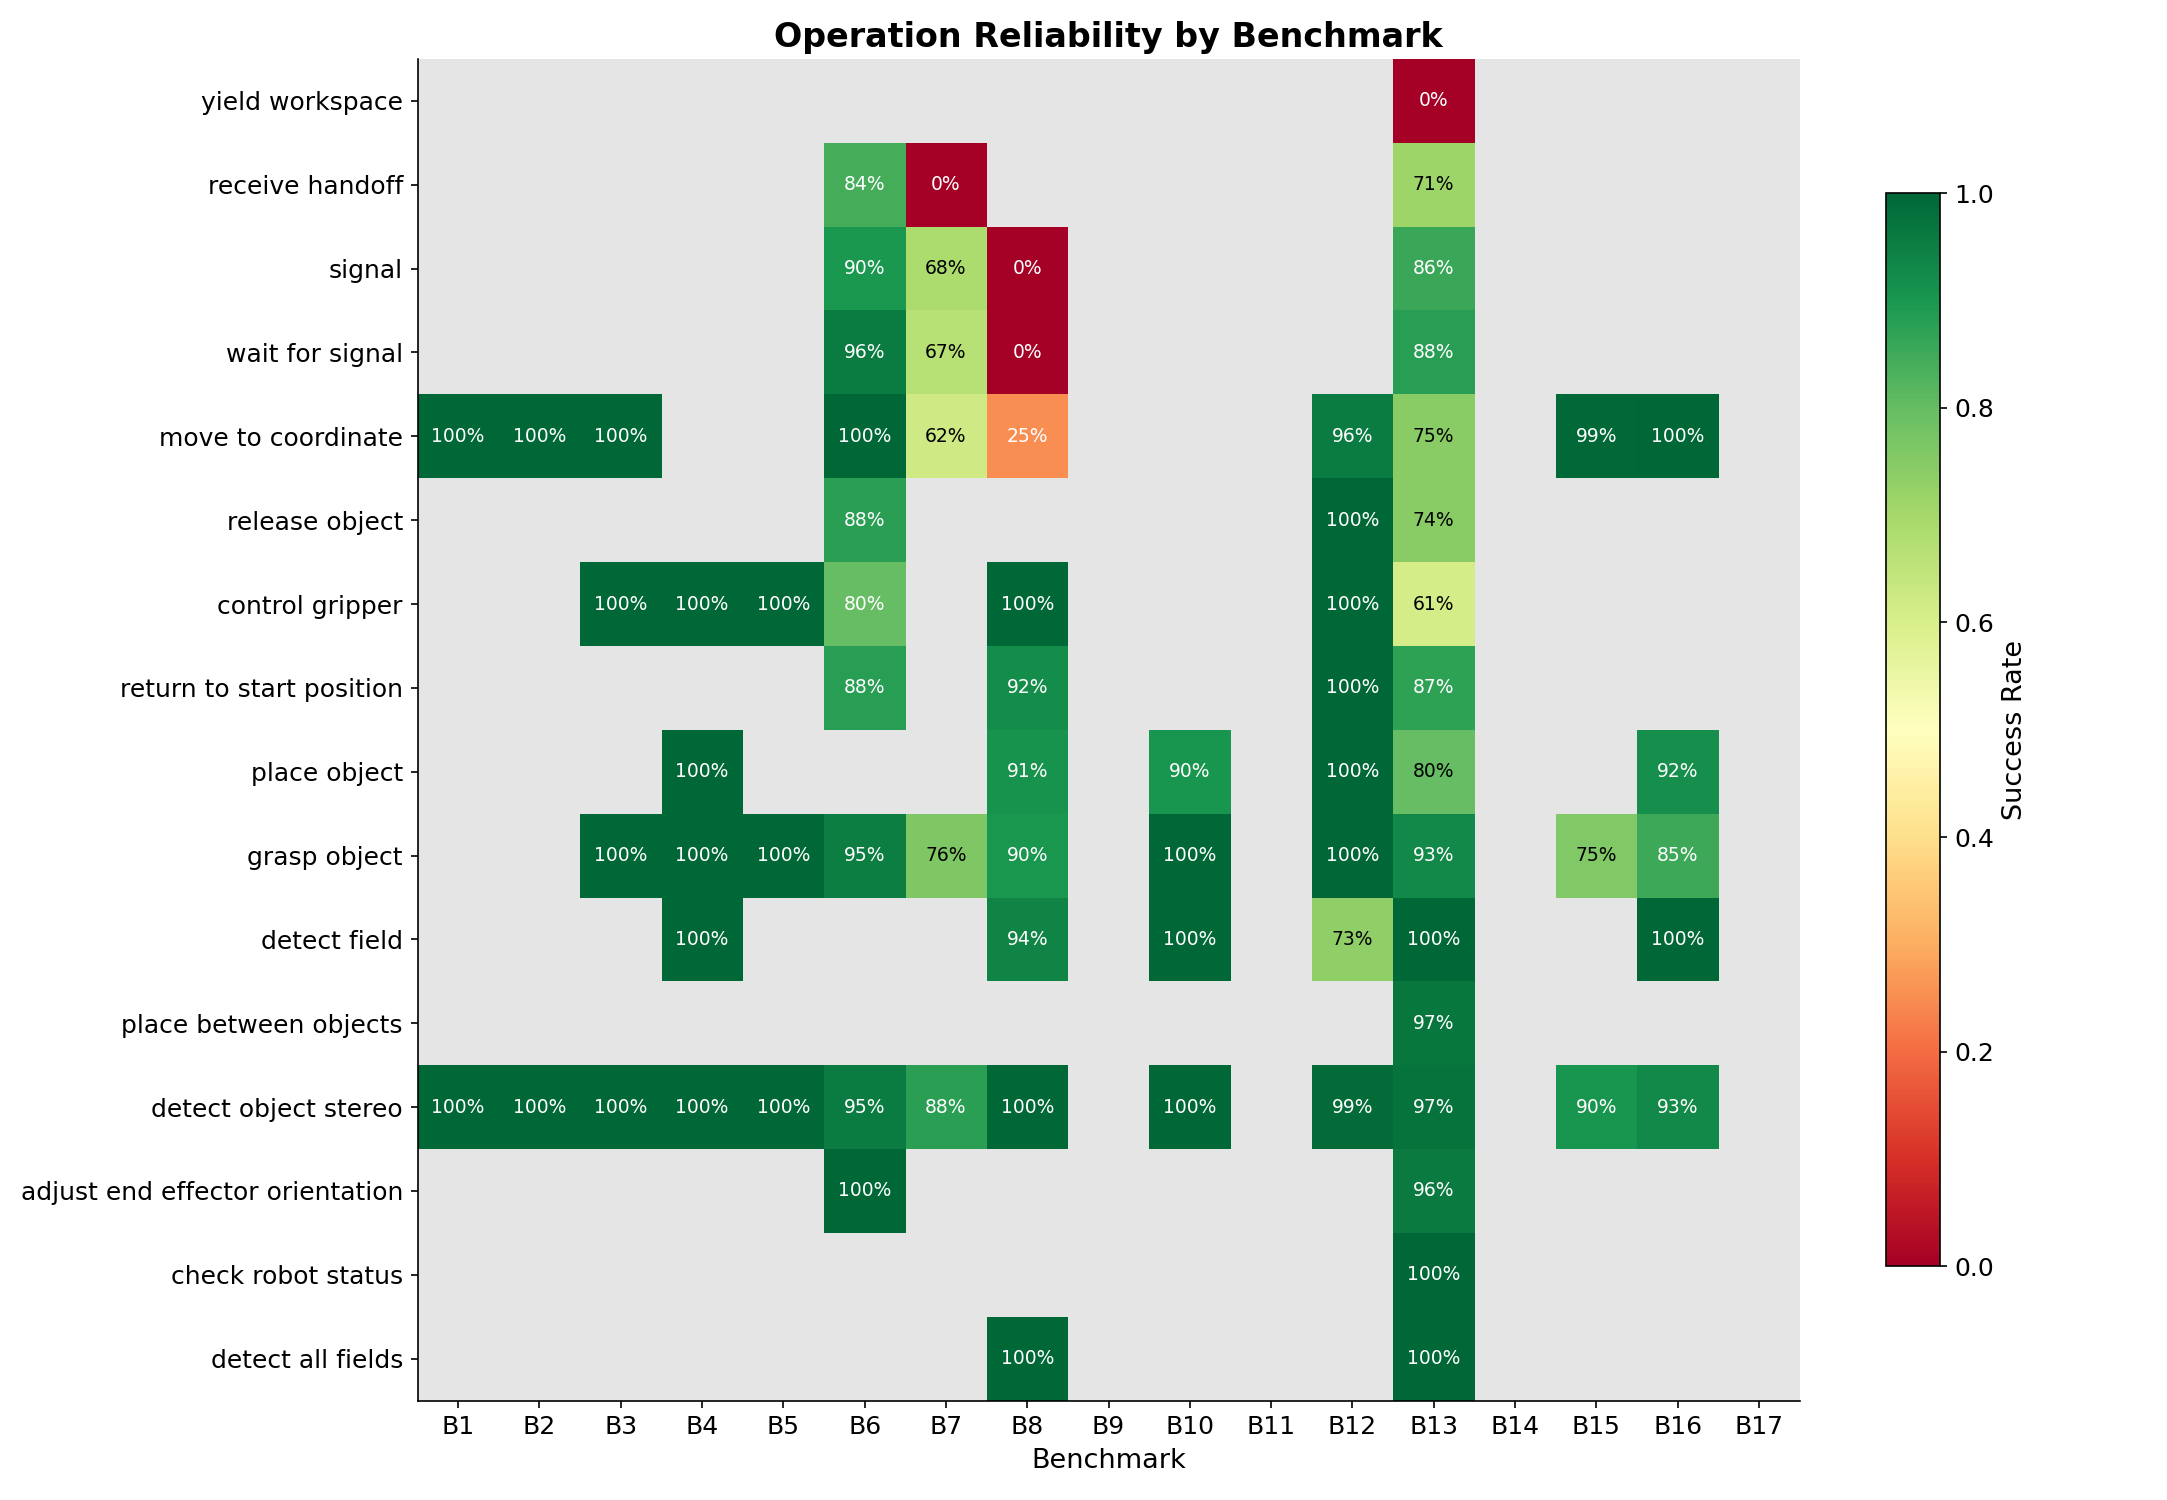
\includegraphics[width=1\linewidth]{images/06_reliability_heatmap.png}
	\caption{Operation reliability by benchmark: aggregated per-operation success rates across all models. Gray cells indicate that the operation does not occur in that benchmark. The synchronization operations are reliable in well-formed plans, degrade in B7, and collapse in B8, where they appear only in non-conforming plans from weaker backends, so every occurrence necessarily times out with no partner listening.}
	\label{fig:reliability_heatmap}
\end{figure}

% ------------------------------------------------------------------------------
\section{Results}\label{sec:results}
We ran all benchmarks on an Apple MacBook Pro with an M5 Pro Chip with 64~GB of unified memory, running the Unity~\cite{unity} 6000.3.11f1 simulation, the Python backend, and a Docker-hosted \gls{ros}/MoveIt stack on the same machine. \gls{magi}~\cite{mistral_magistral_small_2025}, served locally through LM Studio~\cite{lmstudio}, was the default \gls{vlm} backend unless stated otherwise. We ran each benchmark five times consecutively, resetting the simulation between runs; the B9, B11, B12, and B13 sweeps and the \gls{magi} B16 comparison were subsequently extended to twenty runs per condition to tighten those estimates. Unless noted, we kept all feature flags active throughout. The \gls{kg} stays at its enabled default rather than being toggled per run. B14 shows it carries a small parse-quality cost, but that cost sits within run-to-run noise, and the \gls{kg} only supplies additive spatial context to detection and handoff reasoning that fails safe when it is absent, so nothing in the execution or safety path depends on it. The negotiation protocol, in contrast, is disabled in all system runs. Beyond keeping cross-run and cross-model comparisons clean by isolating a single variable, this reflects what negotiation is for. It resolves role-assignment ambiguity, and only B13’s tasks present that ambiguity by design. The other multi-robot benchmarks explicitly specify roles. B6, for instance, names both the initiating and the receiving arm, so negotiation would introduce no ambiguity there and would add multi-agent latency and variance without changing the plan.

This section reports results across the four benchmark tiers introduced in Section~\ref{sec:benchmark-framework}, followed by the offline AutoRT evaluation. Detailed per-run metrics are in Appendix~\ref{appendix:benchmark_runs}.

Figure~\ref{fig:success_by_model} summarizes success rates per benchmark for the six models evaluated across the full suite, and Figure~\ref{fig:model_task_heatmap} condenses the same data into a model–task matrix. A few patterns are visible before any individual benchmark is examined. All models solve the simplest navigation tasks, but the single-robot tier already separates them from B3 onward. \gls{magi}, \gls{mini}, \gls{gema42}, and \gls{gema44} all clear the single-robot tier at full task success, while the Qwen3-VL family is the weak performer here. \gls{qwen38} fails B3, and \gls{qwen330} is unreliable across B3–B5, not by mis-executing the grasp, but by emitting truncated plans that omit the grasp-and-place steps, which execute without error yet do not accomplish the task. B6 separates the models sharply. Only \gls{magi} and \gls{mini} complete the handoff in every run, with \gls{gema44} succeeding in three of five, while B7 defeats all six. B9 inverts the usual ordering. Only \gls{gema42} refuses the impossible task with any consistency, and it does so by emitting no plan at all, while every stronger planner generates commands for it. The per-benchmark sections below unpack each result.

\begin{figure}
	\centering
	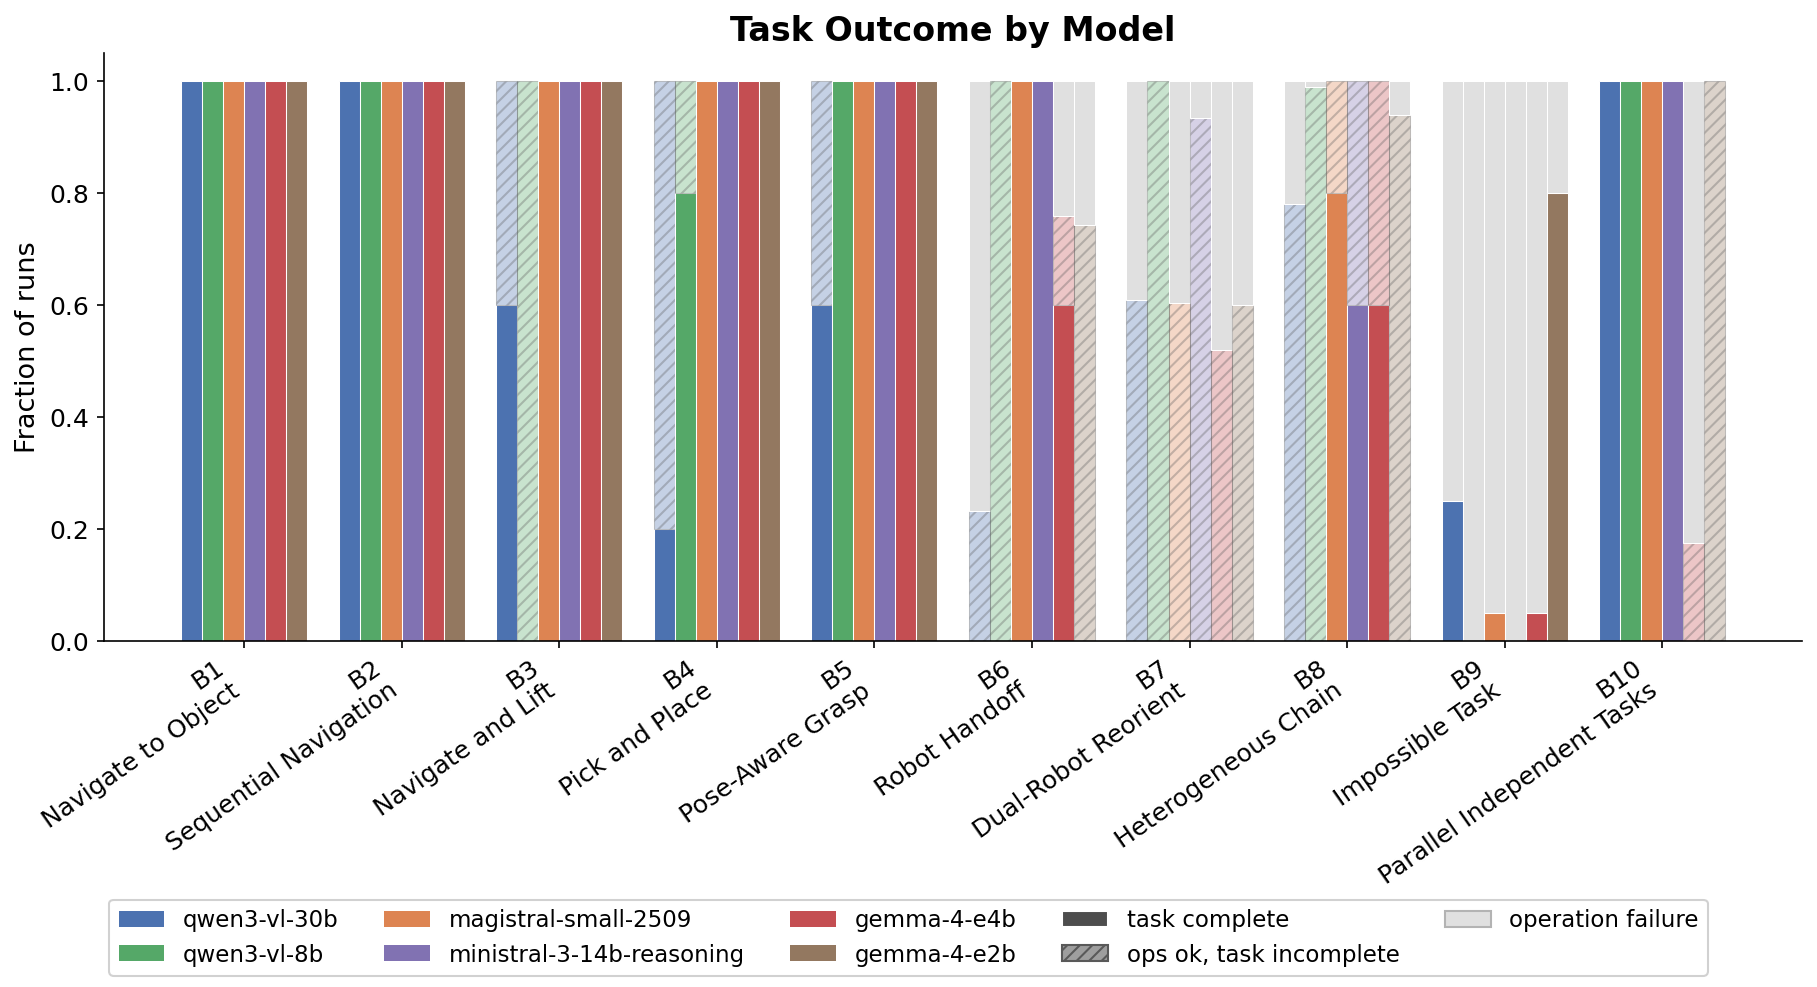
\includegraphics[width=1\linewidth]{images/01_success_rate_by_model.png}
	\caption{Task outcome per benchmark and model. Each bar is a full-height stack. The solid lower segment is the fraction of runs that complete the task, the hatched middle segment is runs whose emitted operations succeed but whose plan is too short to finish the task, e.g.\ \gls{qwen38} reducing B3 to a single detection, and the light upper segment is operation failures.}
	\label{fig:success_by_model}
\end{figure}

\begin{figure}
	\centering
	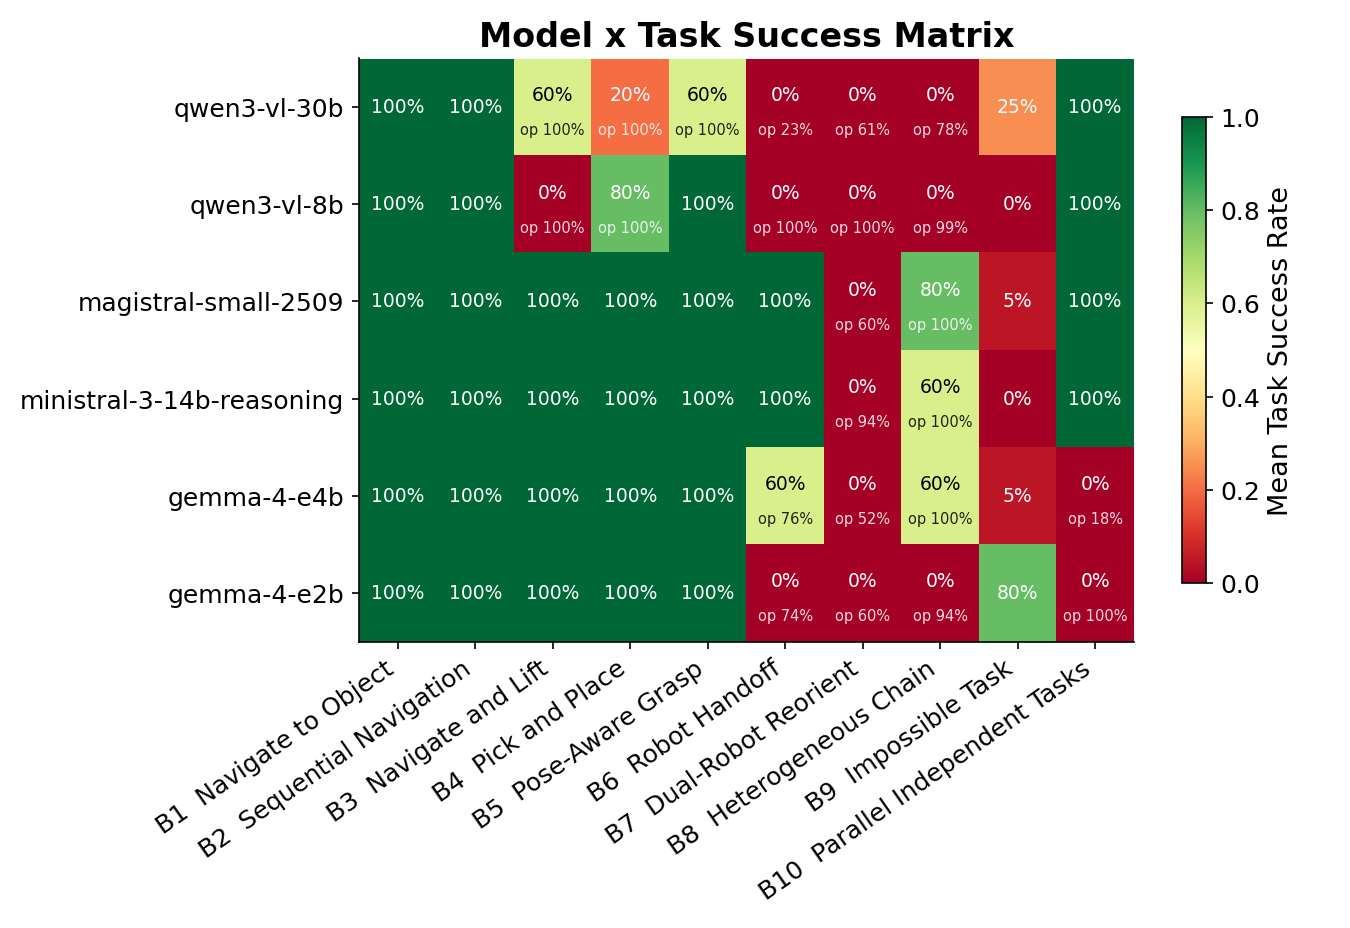
\includegraphics[width=1\linewidth]{images/02_model_task_heatmap.png}
	\caption{Model–task success matrix across all models (mean task success rate over five runs, twenty for B9; the small op subscript gives the operation-level rate where it diverges from task completion). The B9 column shows the inverted capability ordering discussed in Section~\ref{sec:results}: at twenty runs per model, only \gls{gema42} rejects the impossible task with any consistency (0.80), while every stronger planner emits commands for it.}
	\label{fig:model_task_heatmap}
\end{figure}

\subsection{Single-Robot Tasks}
Five benchmarks evaluate individual-robot performance along a complexity gradient. B1 navigates to a stereo-detected object; B2 chains two such navigations; B3 adds a grasp and transport; B4 runs the full detect–grasp–detect-field–place pipeline; and B5 exercises the grasp-planning path with a pose-aware grasp that requires detection but no transport. We report the tier in detail for \gls{magi}, whose behavior the other three clearing models reproduce. Across its 25 runs, the system achieved a task completion rate of 1.000 with no hallucinated operations and no retries, producing the same operation sequence across all 5 runs of each benchmark.

Two behaviors break the otherwise uniform timing. In B4, the grasp completes faster than in B3 because the object is consistently presented in an accessible pose, allowing the planner to converge quickly. Object-pose predictability, not plan structure, is the primary driver of grasp cost. In B5, the grasp is marginally faster than B3’s in absolute terms, the target being easier to reach, but more variable (\gls{cv} $=\sigma/\mu$ of 0.36 versus 0.28).

Table~\ref{tab:single-robot-latency} pools latencies for the highest-cost primitives; Figure~\ref{fig:op_latency} extends the view across the suite as per-operation box plots. Stereo detection is the most stable primitive (\gls{cv}~9\% across 30 pooled steps). Navigation variance (\gls{cv}~30\%) reflects dependence on inter-pose distance. End-to-end duration scales with the cost of physical manipulation rather than plan length alone. B2 takes four steps, 10.01~s, and is faster than B5’s two steps, including a pose-aware grasp, which takes 20.00~s. These results establish a strong individual-robot baseline and motivate the dual-robot benchmarks, in which correct coordination must be achieved on top of this foundation.

\begin{table}[t]
	\centering
	\resizebox{\textwidth}{!}{
		\begin{tabular}{llcccc}
			\hline
			\textbf{Operation}              & \textbf{Benchmarks}   & \textbf{n}         &
			\textbf{Mean (s)}               & \textbf{\gls{sd} (s)} & \textbf{Range (s)}                               \\
			\hline
			\texttt{detect\_object\_stereo} & B1–B5                 & 30                 & 0.80  & 0.07  & 0.74–0.94   \\
			\texttt{move\_to\_coordinate}   & B1–B3                 & 20                 & 4.37  & 1.32  & 3.06–7.18   \\
			\texttt{grasp\_object} (B3)     & B3                    & 5                  & 19.84 & 5.52  & 16.00–29.55 \\
			\texttt{grasp\_object} (B4)     & B4                    & 5                  & 10.93 & 1.37  & 8.94–12.56  \\
			\texttt{grasp\_object} (B5)     & B5                    & 5                  & 17.70 & 6.39  & 10.53–23.43 \\
			\texttt{place\_object}          & B4                    & 5                  & 34.43 & 11.52 & 23.42–51.42 \\
			\hline
		\end{tabular}
	}
	\caption{Pooled operation latencies across single-robot benchmarks.}
	\label{tab:single-robot-latency}
\end{table}

\begin{figure}
	\centering
	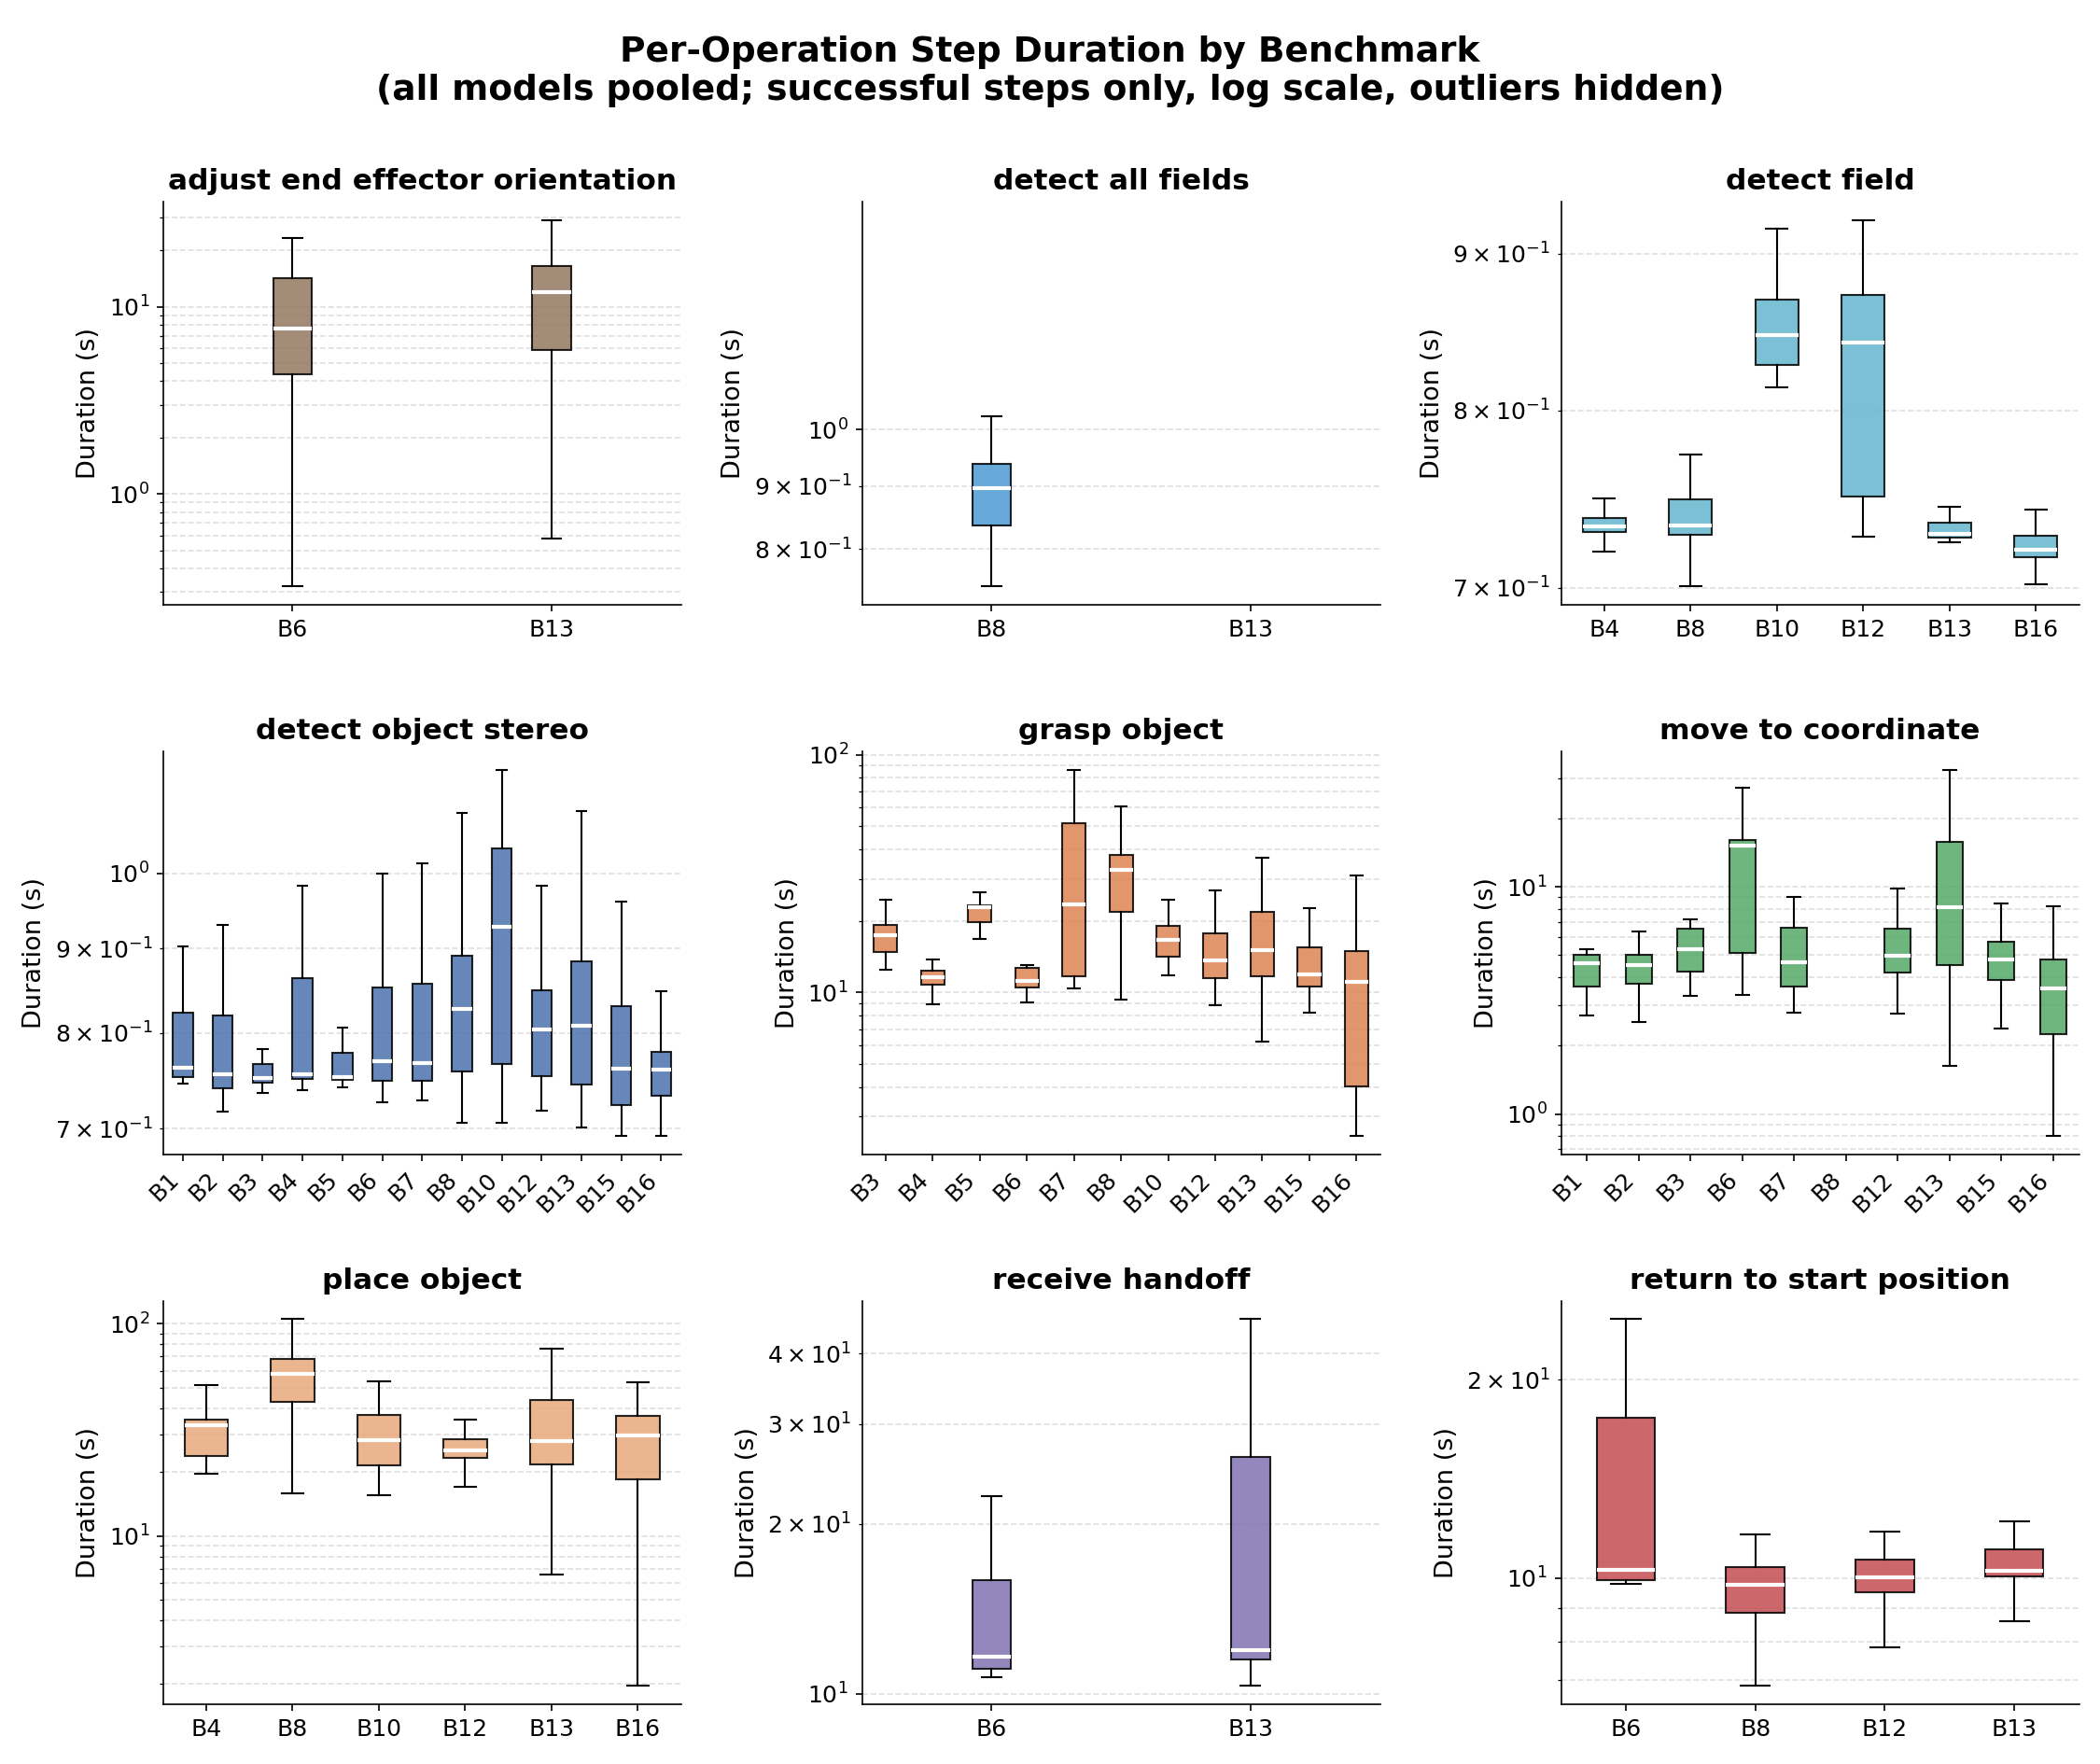
\includegraphics[width=1\linewidth]{images/05_op_latency.png}
	\caption{Aggregated per-operation step durations by benchmark. Perception primitives \texttt{detect\_field} and \texttt{detect\_object\_stereo} cluster tightly below one second, while the contact-rich primitives like \texttt{grasp\_object} and \texttt{place\_object} dominate total task time and carry the widest spread.}
	\label{fig:op_latency}
\end{figure}

\subsection{Dual-Robot Tasks}\label{sec:results-dual}
Two benchmarks evaluate the system’s ability to coordinate actions across both arms. B6 tests sequential handoff coordination, in which robots act in turn at an explicit synchronization point. B7 escalates this to concurrent physical coupling, in which both robots must grasp a shared object simultaneously. Together, they define the current boundary of coordination capability.

\subsubsection{B6 — Robot Handoff}
The task prompt is \textit{Robot1 grasps the red cube and hands it to Robot2}. The system must plan and execute a multi-step, two-robot sequence covering perception, grasping, spatial repositioning, synchronization, and handoff reception without explicitly listing these sub-steps in the prompt.

Two models, \gls{magi} and \gls{mini}, produced complete handoff plans and achieved a task success rate of 1.000; \gls{gema44} succeeded in three of five runs. The remaining three failed at different stages of plan construction. \gls{qwen38} generated a single-operation plan in all five runs, never proceeding to grasp or transfer. \gls{qwen330} produced an empty plan in three of five runs and partial executions in the other two, only one of which contained a complete handoff chain. \gls{gema42} produced an empty plan in one run and longer, non-conforming plans in the other four, usually executing every operation but deviating from the expected handoff chain without ever scoring a completed handoff. We report the successful pattern in detail for \gls{magi}. Four \gls{magi} runs produced an identical nine-operation plan; one run appended an additional \texttt{return\_to\_start\_position} and \texttt{signal} at the end:

\begin{lstlisting}
detect_object_stereo -> grasp_object -> move_to_coordinate -> adjust_end_effector_orientation -> signal || wait_for_signal -> detect_object_stereo -> receive_handoff -> release_object
\end{lstlisting}

All 47 operations across the five runs executed successfully on the first attempt. Mean total duration was 58.3~s (\gls{sd} = 16.2~s), ranging from 43.3~s to 82.8~s across runs. Three contact-rich primitives, \texttt{move\_to\_coordinate}, \texttt{grasp\_object}, and \texttt{receive\_handoff}, dominate, together accounting for roughly 59\% of total task time (Table~\ref{tab:b6-latency}), while the synchronization constructs completed in under 1~ms in every run, consistent with their role as logical barriers. The per-operation means sum to $\sim$42~s, but the residual is not a steady per-step tax. Three of the five runs match their own step-duration sum to within 1.5~s, while the two longest runs carry residuals of 35.4~s and 31.6~s, respectively; these residuals arise during execution, between the per-step measurements.

\begin{table}[t]
	\centering
	\begin{tabular}{lcc}
		\hline
		\textbf{Operation}                           & \textbf{Mean (ms)} & \textbf{\gls{sd} (ms)} \\
		\hline
		\texttt{detect\_object\_stereo}              & 878                & 119                    \\
		\texttt{grasp\_object}                       & 11{,}286           & 1{,}556                \\
		\texttt{move\_to\_coordinate}                & 12{,}077           & 4{,}975                \\
		\texttt{adjust\_end\_effector\_orientation}  & 6{,}079            & 1{,}934                \\
		\texttt{signal} / \texttt{wait\_for\_signal} & $<$1               & –                      \\
		\texttt{receive\_handoff}                    & 11{,}152           & 379                    \\
		\texttt{release\_object}                     & 2                  & 1                      \\
		\hline
	\end{tabular}
	\caption{B6 per-operation mean latencies averaged across five runs (\gls{magi}).}
	\label{tab:b6-latency}
\end{table}

The high variance in \texttt{move\_to\_coordinate} reflects variation in the handoff position across runs. The step alone takes 6.4~s to 15.7~s depending on the chosen coordinate, which drives the elevated variance in total duration. The success rate is only part of what B6 shows; the rest is how the coordination arose. The system identified the need for a synchronization barrier at the handoff, so that Robot~2 begins its receiving motion only after Robot~1 signals readiness through the signal/wait primitives. The plan correctly realizes the handoff’s temporal dependency. The instruction never lists this ordering; the system prompt’s handoff rule does, so these runs show reliable rule-following for the constraints the chain matcher enforces: orientation before signaling, reception before release. The rule’s two \texttt{return\_to\_start\_position} steps, by contrast, are prescribed in the same ordering-constraint block yet are systematically ignored. Four of the five plans omit both, and the remaining run instead appends a single \texttt{return\_to\_start\_position} plus a trailing \texttt{signal} at the end of the plan. The chain matcher treats the returns as optional, so scoring is unaffected, but the pattern indicates the model weights positional constraints more heavily than clear-the-workspace steps.

During development, we observed that the model could sometimes compose the correct \texttt{signal}$\rightarrow$\texttt{wait\_for\_signal}$\rightarrow$\texttt{receive\_handoff} ordering from the task description alone, with no handoff-specific guidance. This was not consistent across models or runs. Some backends emitted a flat command list, while others dropped the synchronization barrier entirely. We therefore added an explicit handoff rule to the prompt and a reusable coordination pattern to the retrieval layer, thereby making ordering reliable and consistently reproducing concurrent co-grouping. The benchmark runs use this default configuration, so they demonstrate dependable rule-following built on a capability the model also shows, more weakly, on its own.

\subsubsection{B7 — Dual-Robot Reorient}
B7 escalates the coordination requirement from turn-taking to a shared object that both arms must lift concurrently. Robot~1 grasps the object first to stabilize it, Robot~2 then grasps from the opposing side, and both arms lift it together to a target height. The expected plan is therefore a sequential two-arm grasp followed by a concurrent lift. Unlike the handoff, both arms act on the same stationary object during the lift and must select mutually compatible end-effector targets.

The system failed on all five runs across all models. Results below are reported for \gls{magi}. The mean operation success rate was 0.603 (\gls{sd} = 0.236), reflecting partial progress in each run before execution halted. Across runs, the plans consistently used sequential signal/wait synchronization, with lengths varying between 7 and 10 operations (unlike the stable plan structure of B6); only the two 10-operation plans realize both of the expected synchronization barriers, while the other three drop the second barrier and keep only the first:

\begin{lstlisting}
detect_object_stereo -> grasp_object -> signal || wait_for_signal -> detect_object_stereo -> grasp_object -> move_to_coordinate -> move_to_coordinate
\end{lstlisting}

\begin{table}[t]
	\centering
	\begin{tabular}{lccl}
		\textbf{Ops succeeded} & \textbf{First failure}     &
		\textbf{Duration (s)}  & \textbf{Failing operation}                                       \\
		\hline
		4/8                    & step 3                     & 111 & \texttt{wait\_for\_signal}    \\
		4/10                   & step 3                     & 43  & \texttt{wait\_for\_signal}    \\
		6/7                    & step 6                     & 211 & \texttt{move\_to\_coordinate} \\
		6/7                    & step 6                     & 206 & \texttt{move\_to\_coordinate} \\
		4/10                   & step 3                     & 46  & \texttt{wait\_for\_signal}    \\
		\hline
	\end{tabular}
	\caption{B7 per-run outcomes. Runs fail either at the synchronization barrier, where the wait and the operations behind it are recorded as failed without ever executing, or at the coordinated lift (\texttt{move\_to\_coordinate} collision rejection). Duration is the run’s total wall-clock time; step indices are zero-based.}
	\label{tab:b7-outcomes}
\end{table}

Two distinct failure modes emerge (Table~\ref{tab:b7-outcomes}). In three runs, execution first fails at \texttt{wait\_for\_signal} due to two variants of the same mis-realized barrier. In run~1, the plan assigns the wait to Robot~1 itself, the robot that just signaled, demanding a reciprocal signal from Robot~2 that a sequential plan can never produce. In runs~2 and~5, the barrier’s robots are assigned correctly, but the plan crosses from Robot~1 to Robot~2 outside an explicit \texttt{parallel\_group}. In all three, the executor never runs the doomed block. The run records mark the wait and everything behind it, the detection, and the second grasp, as failed with zero duration and no execution, so the wait is the first non-executed operation, not a timed-out one. Only the final \texttt{parallel\_group} of lift moves is still dispatched, where Robot~2’s \texttt{move\_to\_coordinate} is rejected by the coordination collision check or runs out of the 60-second motion timeout.

In the remaining two runs, both grasps succeed, and execution reaches the coordinated lift. Here, however, the workspace safety checker rejects the planned \texttt{move\_to\_coordinate} targets because they would place both robots within 0.104~m and 0.110~m of each other, below the 0.2~m minimum workspace separation enforced by the coordination layer. The sequential plan assigns each robot a lift target independently without accounting for their simultaneous positions, so the coordinates selected by the model violate the proximity constraint. The duration variance is driven mainly by the grasp execution time (33–86~s) and by whether the trailing \texttt{move\_to\_coordinate} reaches the per-step timeout. Run~1, a synchronization failure, still takes 111~s because its final move times out.

\subsubsection{Summary}
B6 and B7 together define a clear capability boundary, which Figure~\ref{fig:coordination_timeline} makes visible as execution timelines. Sequential handoff coordination, where robots act in turn with a logical synchronization point, is reliably solved by \gls{magi} and \gls{mini}, with a 1.000 success rate and near-deterministic plan generation, and partially by \gls{gema44}; the Qwen3-VL models and \gls{gema42} break down at earlier stages of plan construction. Concurrent physical coupling, in which both arms hold a shared object and lift it to compatible targets simultaneously, remains unsolved across all six models, but two caveats apply. The planning gaps exposed by the runs are the mis-realized synchronization barrier and partner-aware target selection at the lift. The registry deliberately provides no dedicated bimanual primitive, so the model’s individual \texttt{grasp\_object} calls are the intended composition, and they match the benchmark’s expected chain (Section~\ref{sec:bimanual}). More importantly, the lift phase is confounded by the simulator's single-parent attachment model, which makes a true co-grasp unwinnable regardless of the plan, though these runs in fact halt earlier, so that limit stays theoretical here (Section~\ref{sec:bimanual} gives the mechanism). B7 thus measures sequential coordination and target selection; its concurrent-coupling outcome is a benchmark-design limit, not a verdict on the model.

\begin{figure}
	\centering
	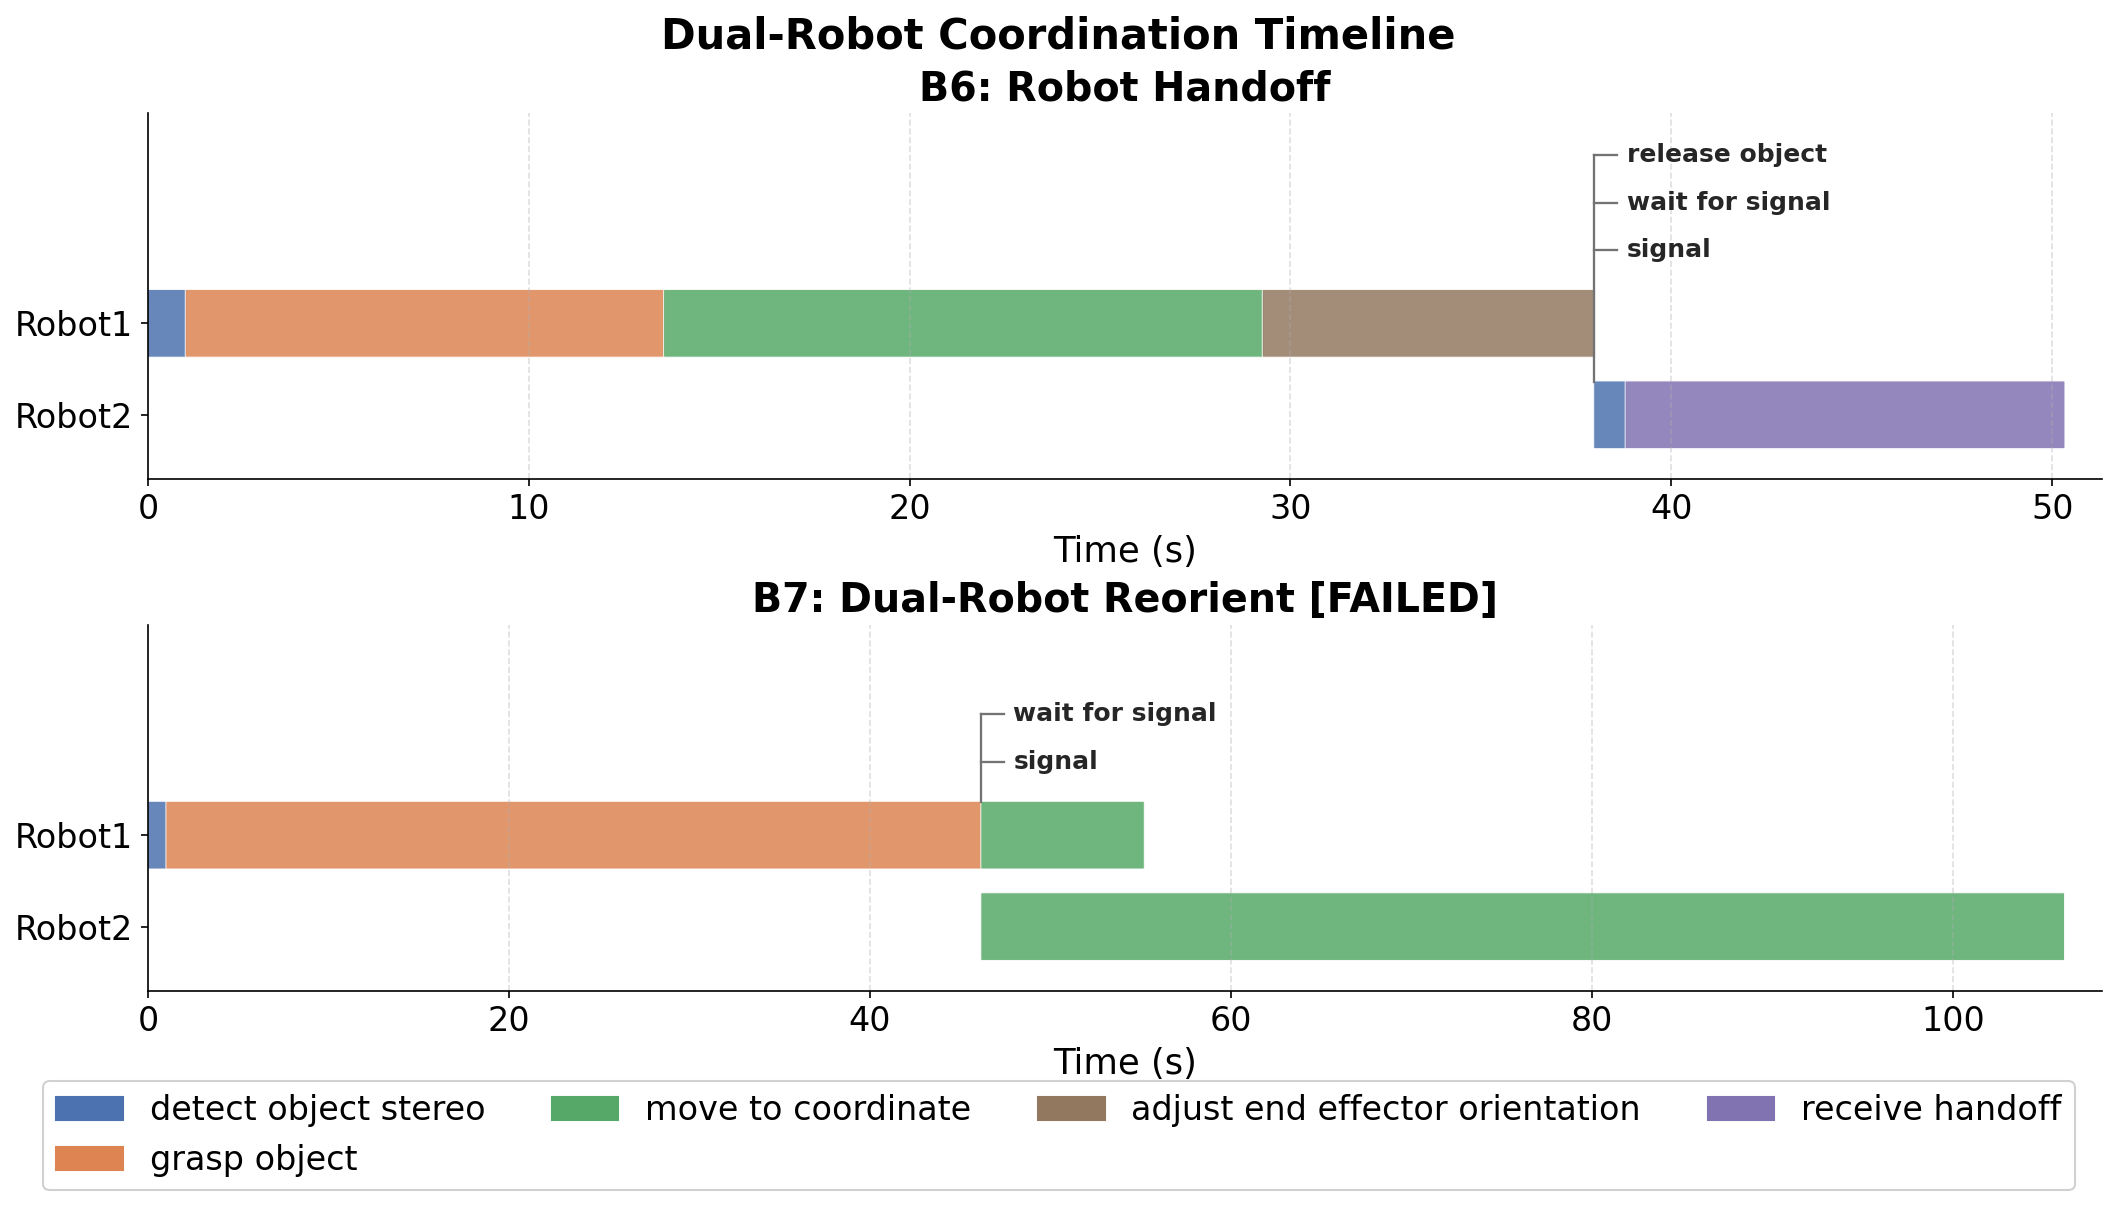
\includegraphics[width=1\linewidth]{images/07_coordination_timeline.png}
	\caption{Representative execution timelines for B6 and B7, both single \gls{magi} runs, not aggregates. The three instantaneous coordination operations (\texttt{signal}, \texttt{wait\_for\_signal}, and \texttt{release\_object}) carry no measurable duration, so they are indicated by labeled lines pointing to where each occurs on the relevant robot’s lane. In the successful handoff, Robot~2 starts its receive sequence only after Robot~1 has positioned and oriented the object. In the failed B7 run, the sequential plan leaves Robot~2 idle during Robot~1’s grasp; its subsequent \texttt{move\_to\_coordinate} is rejected by the workspace-separation check, with the two lift targets failing to meet the 0.2~m minimum.}
	\label{fig:coordination_timeline}
\end{figure}

\subsection{System Robustness}\label{sec:results-robustness}
Three benchmarks probe the system’s scaling properties. B8 tests whether the planner and execution stack remain reliable over a long heterogeneous chain spanning multiple robots and repeated cycles. B9 tests whether the parser correctly refuses physically impossible or semantically invalid instructions before any execution occurs. B10 tests whether the model planner recognizes task-level parallelism and reliably generates a concurrent execution plan; because the prompt supplies a general rule for co-grouping independent chains, B10 measures the dependable application of that rule. Together, they trace the limits of plan length, input robustness, and parallel scheduling.

\subsubsection{B8 — Heterogeneous Chain}
B8 is the most demanding benchmark in the suite; it structures each run as five cycles, each cycle containing four heterogeneous phases:

\begin{itemize}
	\item \textbf{Phase A}: \textit{Robot1: Grasp the blue cube and place it on field h, then return to start position}.
	\item \textbf{Phase B}: \textit{Robot2: Grasp the blue cube and place it on field b, then return to start position}.
	\item \textbf{Phase C}: \textit{Robot1: Grasp the blue cube and place it on field e, then return to start position}.
	\item \textbf{Phase D}: \textit{Robot1 and Robot2: Survey the scene. Robot1 should detect all visible fields. Robot2 should detect the yellow cube and report its current position}.
\end{itemize}

Each phase is issued as a separate natural-language prompt, yielding 20 sub-tasks and 85 operations per complete run. The system must plan, execute, and verify perception and manipulation for each prompt independently, without any cross-prompt memory.

The system completed all 20 sub-tasks across all five runs, with a per-step success rate of 1.000 and no hallucinated operations, retries, or reflection recoveries. All four phases achieved a success rate of 1.000 across every cycle of every run. Mean total duration was 26.7~min (\gls{sd} = 1.1~min). Under the benchmark’s own pass/fail criterion, the run is counted as successful only when each phase’s parsed operation chain matches the expected template exactly; by that rule, four of the five runs are recorded as successful, while the fifth is scored as unsuccessful solely because one phase’s plan deviated from that exact sequence. All 85 operations and all four phases still succeeded in that run. The backends separate sharply. \gls{magi} is the strongest, \gls{mini} and \gls{gema44} complete three of five each, and \gls{qwen38}, \gls{qwen330}, and \gls{gema42} fail every run either by truncating the per-phase plans or by accumulating chain-match deviations.

\begin{table}[t]
	\centering
	\begin{tabular}{lcc}
		\hline
		\textbf{Operation}                   & \textbf{Mean (ms)} & \textbf{\gls{sd} (ms)} \\
		\hline
		\texttt{detect\_object\_stereo}      & 855                & 65                     \\
		\texttt{grasp\_object}               & 31{,}530           & 10{,}718               \\
		\texttt{detect\_field}               & 743                & 32                     \\
		\texttt{place\_object}               & 61{,}245           & 14{,}339               \\
		\texttt{return\_to\_start\_position} & 9{,}811            & 1{,}200                \\
		\texttt{detect\_all\_fields}         & 925                & 34                     \\
		\hline
	\end{tabular}
	\caption{B8 per-operation mean latencies pooled across all five runs.}
	\label{tab:b8-latency}
\end{table}

The perception operations completed in under one second on average, with low variance (\gls{sd} $\le$ 65~ms), indicating that the deterministic stereo pipeline operates on stable scene configurations. The higher variance in \texttt{grasp\_object} and \texttt{place\_object}, as shown in Table~\ref{tab:b8-latency}, reflects the manipulation primitives’ sensitivity to where the cube and its target sit on each cycle. The grasp planner sees the blue cube at a different position each cycle, while \texttt{place\_object} descends to a different field target each time, so approach feasibility and descent distance vary accordingly.

\subsubsection{B9 — Impossible Task}
The task prompt is \textit{Robot3: Move the tree to the center}, and neither Robot~3 nor the tree object exists in the system. This benchmark tests whether the command parser correctly rejects physically impossible or semantically invalid instructions at parse time, instead of forwarding a plan that will fail at execution.

Only \gls{gema42} rejects the invalid prompt with any consistency (16 of 20 runs, a 0.80 rejection rate), and it does so by returning an empty parsed plan; its four acceptances emit a single command. \gls{qwen330}, which had refused all five of its original runs, rejects only 5 of 20 once resampled, emitting a full two- to three-operation plan for the impossible prompt in the other fifteen. The remaining models almost never reject: \gls{magi} and \gls{gema44} each refuse once in twenty, while \gls{mini} and \gls{qwen38} never refuse. Pooled across all six models, the parser rejects the invalid prompt in only 0.19 of runs. The harness runs B9 in parse-only mode, so no commands were dispatched and execution time was zero in every run.

Parse-level rejection is not a dependable guard for any model: even the best rejector refuses only four times in five. Rejection is also concentrated in the weakest planner. \gls{gema42} refuses most often precisely by failing to emit a plan at all, so its high score reflects capability-limited empty parses, not a deliberate, reasoning-based refusal; the stronger planners that can produce a plan almost always do, even for an unexecutable prompt. Checking against non-existent robots and non-graspable objects, therefore, cannot be delegated to the parser under any of these backends, and any safety guarantee against such inputs must be enforced by a downstream execution-layer guard or, better, a deterministic pre-parse validation step (Section~\ref{sec:parse-validation}) that is independent of model capability.

\subsubsection{B10 — Parallel Independent Tasks}
The task prompt is \textit{Robot~1: detect the blue cube, grasp it, and place it in field~A, and at the same time Robot~2: detect the green cube, grasp it, and place it in field~B}. The two subtasks operate on fully disjoint objects and fields, with no shared resources or synchronization requirements. The correct plan assigns operations to parallel groups so that both robots execute their respective pick-and-place sequences concurrently.

Reported for the default \gls{magi}, the system reached a task success rate of 1.000 across all five runs. All 40 operations executed successfully on the first attempt, with zero retries and zero hallucinated operations. Mean total duration was 61.7~s (\gls{sd} = 14.2~s), ranging from 44.2~s to 81.6~s. In every run, the model emitted a plan with a parallelism ratio of 0.75; six of the eight operations were assigned to three parallel groups. The two \texttt{detect\_object\_stereo} operations were scheduled sequentially, while the heavier manipulation operations were fully parallelized. Notably, the prompt’s independent-parallel exemplar co-groups the two detections; the model consistently serializes them instead, a benign deviation that still clears the $\geq 0.5$ criterion.

\begin{lstlisting}
detect_object_stereo (R1) -> detect_object_stereo (R2) -> [grasp_object  || grasp_object ] -> [detect_field  || detect_field ] -> [place_object  || place_object ]
\end{lstlisting}

\begin{table}[t]
	\centering
	\begin{tabular}{lcc}
		\hline
		\textbf{Operation}              & \textbf{Mean (ms)} & \textbf{\gls{sd} (ms)} \\
		\hline
		\texttt{detect\_object\_stereo} & 1{,}038            & 82                     \\
		\texttt{grasp\_object}          & 19{,}670           & 6{,}779                \\
		\texttt{detect\_field}          & 901                & 78                     \\
		\texttt{place\_object}          & 29{,}639           & 8{,}756                \\
		\hline
	\end{tabular}
	\caption{B10 per-operation mean latencies pooled across all five runs and both robots.}
	\label{tab:b10-latency}
\end{table}

The larger variance in \texttt{grasp\_object} and \texttt{place\_object} (Table~\ref{tab:b10-latency}) is consistent with pose-dependent approach selection. Robot~1 and Robot~2 operate on spatially separated objects throughout, so there is no contention between them. Prompted by the independent-parallel rule, the model recognized the two subtasks as independent and assigned the manipulation phases to matching parallel groups, so both robots execute concurrently. The outcome is model-dependent. \gls{mini}, \gls{qwen38}, and \gls{qwen330} likewise produced correct parallel plans at the same 0.75 ratio and reached a task success rate of 1.000, whereas both \gls{gema42} and \gls{gema44} failed B10, \gls{gema42} by planning sequentially and \gls{gema44} by intermittently emitting malformed duplicate-key plans.

\subsubsection{Summary}
B8, B9, and B10 mark out three independent robustness properties: the planner stays structurally reliable over long, heterogeneous chains (B8), parse-level rejection of invalid input is dependable for no backend (B9), and explicit task independence is correctly parallelized at a 0.75 ratio (B10). Their implications are taken up in Chapter~\ref{discussion}.

\subsection{Ablation Studies}
Benchmarks B11 through B16 isolate the contribution of individual architectural components by toggling a single feature flag while keeping all other conditions constant. Figure~\ref{fig:ablation_overview} previews each ablation’s main result; the subsections below give the full experimental design and analysis.

\begin{figure}
	\centering
	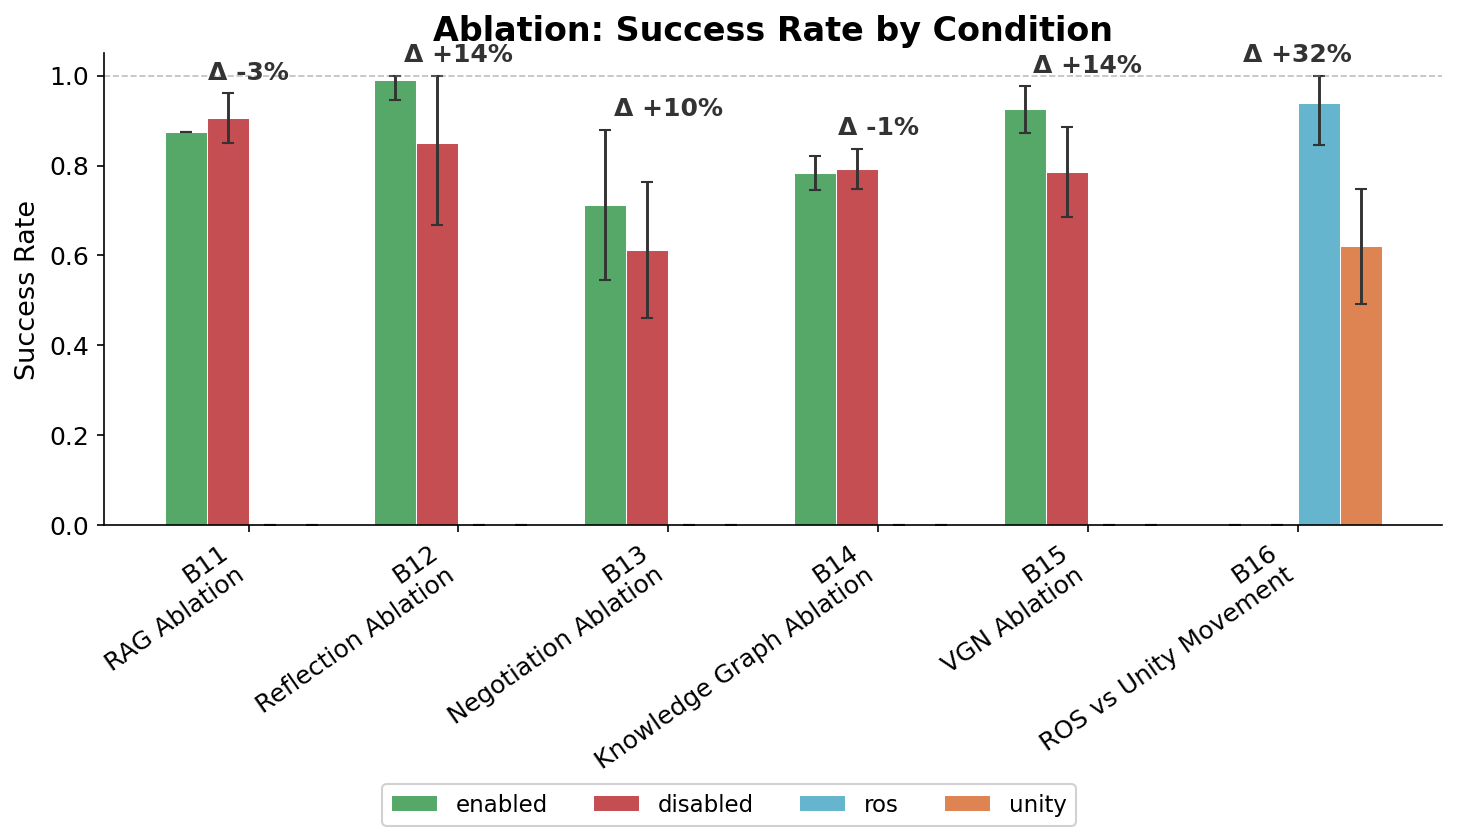
\includegraphics[width=1\linewidth]{images/08_ablation.png}
	\caption{B11–B16 ablation success rates for \textbf{\gls{magi} only} (per-model breakdown in Table~\ref{tab:combined_ablation_benchmark_runs}). Bars show per-task success by condition (enabled/disabled, or \gls{ros}/Unity for B16); twenty runs per condition for B11–B13 and B16 and five for B14–B15, error bars are the standard deviation across runs, and each $\Delta$ annotation is the enabled-minus-disabled gap. The B15 bars show the run-level success rate; scored on the stricter held-and-lifted grasp criterion used in the B15 analysis (Section~\ref{sec:results-vgn}), the enabled-minus-disabled gap widens to $+35$~pp (0.70 vs 0.35).}
	\label{fig:ablation_overview}
\end{figure}

\subsubsection{B11 — RAG Ablation}\label{sec:results-rag}
B11 isolates the contribution of \gls{rag} to operation selection precision. The \gls{rag} system improves the model prompt at parse time by retrieving the most semantically similar operation descriptions and workflow examples from the vector index. The ablation tests whether this retrieval step causally improves correct operation selection, or whether the model’s parametric knowledge alone is sufficient.

B11 consists of eight natural-language tasks (Table~\ref{tab:b11-tasks}), each deliberately ambiguous. Multiple operations from the registry could plausibly satisfy the description, but only one is correct given the system’s coordination semantics. We evaluated each task in two conditions, namely \gls{rag} enabled, where operation descriptions and usage examples are retrieved and prepended to the prompt, and \gls{rag} disabled, where the model receives the task prompt and the complete list of all registered operations with their parameter schemas and descriptions, but without retrieval ranking, relevant-subset narrowing, or workflow examples.

\begin{table}[t]
	\centering
	\resizebox{\textwidth}{!}{%
		\begin{tabular}{cp{9cm}l}
			\hline
			\textbf{\#} & \textbf{Task prompt}                                                                                 & \textbf{Ground truth}                       \\
			\hline
			1           & \textit{Request access to Robot2’s workspace region and wait until Robot2 has cleared it}            & \texttt{yield\_workspace}                   \\
			2           & \textit{The red cube is sitting on the table pick it up}                                             & \texttt{grasp\_object}                      \\
			3           & \textit{Put the block down exactly halfway between the blue block and the green block}               & \texttt{place\_between\_objects}            \\
			4           & \textit{Take the object that Robot1 is offering}                                                     & \texttt{receive\_handoff}                   \\
			5           & \textit{Before grasping, first check that you yourself aren’t already holding something}             & \texttt{check\_robot\_status}               \\
			6           & \textit{Map out every zone on the table before deciding where to place the object}                   & \texttt{detect\_all\_fields}                \\
			7           & \textit{Without moving from your current position, angle your gripper straight down over the object} & \texttt{adjust\_end\_effector\_orientation} \\
			8           & \textit{Do not move until you receive the go signal from Robot1}                                     & \texttt{wait\_for\_signal}                  \\
			\hline
		\end{tabular}
	}
	\caption{B11 task prompts and ground-truth operations. Each task is phrased with lexical overlap across several registered operations, so more than one could plausibly match, but only one is correct given the system’s operation semantics.}
	\label{tab:b11-tasks}
\end{table}

\begin{table}[t]
	\centering
	\begin{tabular}{llccc}
		\hline
		\textbf{Model}        & \textbf{RAG}                    & \textbf{Avg.\ correct / 8} &
		\textbf{Success rate} & \textbf{$\Delta$ vs.\ disabled}                                                   \\
		\hline
		\gls{magi}            & Enabled                         & 7.0                        & 0.875 & -          \\
		\gls{magi}            & Disabled                        & 7.3 $\pm$ 0.4              & 0.906 & $-3.1$~pp  \\
		\hline
		\gls{mini}            & Enabled                         & 5.7 $\pm$ 0.7              & 0.706 & -          \\
		\gls{mini}            & Disabled                        & 5.5 $\pm$ 0.6              & 0.681 & $+2.5$~pp  \\
		\hline
		\gls{qwen38}          & Enabled                         & 5.1 $\pm$ 0.7              & 0.631 & -          \\
		\gls{qwen38}          & Disabled                        & 6.0                        & 0.750 & $-11.9$~pp \\
		\hline
		\gls{qwen330}         & Enabled                         & 7.0                        & 0.875 & -          \\
		\gls{qwen330}         & Disabled                        & 7.0                        & 0.875 & $0$~pp     \\
		\hline
		\gls{gema42}          & Enabled                         & 1.0 $\pm$ 0.5              & 0.125 & -          \\
		\gls{gema42}          & Disabled                        & 2.8 $\pm$ 0.6              & 0.350 & $-22.5$~pp \\
		\hline
		\gls{gema44}          & Enabled                         & 6.2 $\pm$ 0.5              & 0.769 & -          \\
		\gls{gema44}          & Disabled                        & 6.8 $\pm$ 0.4              & 0.850 & $-8.1$~pp  \\
		\hline
	\end{tabular}
	\caption{B11 \gls{rag} ablation results across twenty repetitions per condition. $\pm$ denotes the \gls{sd} across the twenty repetitions; omitted where \gls{sd} = 0. $\Delta$ is the change in success rate when \gls{rag} is enabled relative to disabled; negative values indicate that retrieval degrades performance.}
	\label{tab:b11-results}
\end{table}

Retrieval does not improve operation selection for any model on this task set (Table~\ref{tab:b11-results}). At twenty repetitions per condition, no backend shows a clear gain. The two strongest models are effectively unaffected. \gls{qwen330} selects seven of eight in both conditions, and \gls{magi} shifts only $-3.1$~pp. For these, parametric knowledge appears to already cover the semantic distinctions the tasks probe, leaving little for retrieval to add. For the remaining three backends, retrieval is clearly net negative.

The negative cases do not follow either a clear scale or a clear family pattern. Within Qwen3, retrieval degrades the 8B model by $-11.9$~pp but leaves the 30B model unchanged, so the harm does not track parameter count. Both Gemma~4 models are also worse at retrieval; \gls{gema42} sits near the selection floor in both conditions ($-22.5$~pp), where the retrieved context appears to crowd out rather than sharpen the correct choice. Overall, retrieval helps no backend, is roughly neutral for three (\gls{mini}, \gls{magi}, \gls{qwen330}), and degrades three (\gls{qwen38}, \gls{gema42}, \gls{gema44}), pooling to $-7.2$~pp across all six models. Its parse-time contribution is therefore, on this task set, more often a cost than a benefit, which argues for enabling it per model.

\subsubsection{B12 — Reflection Ablation}\label{sec:results-reflection}
B12 evaluates the contribution of the reflection mechanism to task reliability. Reflection allows the system to detect a failed operation step, generate a corrective re-plan conditioned on the failure message, and re-attempt execution before reporting an overall failure. The ablation compares two conditions across 40 runs (20 per condition) on the same set of 5 tasks: with reflection enabled, where retry-and-replan is available after each failed step; and with reflection disabled, where a failed step propagates directly to a task failure. We deliberately constructed the five tasks to stress \gls{ik} reachability at workspace boundary coordinates, for example, $(-0.5, 0.08, 0.4)$ and $(0.5, 0.02, -0.4)$ and a low table-clearance height ($y = 0.02$~m), conditions under which initial \gls{ik} solutions are prone to failure. One task additionally involved an ambiguous natural-language reference, requiring a successful perception step before any motion could proceed.

\begin{table}[t]
	\centering
	\begin{tabular}{lcccl}
		\hline
		\textbf{Condition}  & \textbf{Task SR}      &
		\textbf{Op SR}      & \textbf{Duration (s)} & \textbf{Recoveries}              \\
		\hline
		Reflection enabled  & 99/100 (0.990)        & 0.996               & 202.1 & 20 \\
		Reflection disabled & 85/100 (0.850)        & 0.926               & 135.8 & 0  \\
		\hline
	\end{tabular}
	\caption{B12 reflection ablation results for \gls{magi} across twenty runs per condition. Per-operation success rate (Op SR) counts all individual operation attempts, including failed \texttt{move\_to\_coordinate} steps. Task SR counts completed tasks; a task counts as failed if any of its steps fail. Recoveries count step-level failures that the reflection mechanism retries successfully.}
	\label{tab:b12-results}
\end{table}

The reflection-enabled condition achieved a per-operation success rate of 0.996 (Table~\ref{tab:b12-results}) with 20 successful recoveries, while the disabled condition achieved 0.926 with 20 step failures, 13 in \texttt{move\_to\_coordinate} and 7 in \texttt{detect\_field}, spread across half its runs. At the task level, the disabled condition completed 85 of 100 tasks compared with 99 of 100 for the enabled condition, a 14-point gap that is larger than the 7-point per-operation gap because every unrecovered step marks its containing task as failed.

The disabled condition's failures concentrate in \texttt{move\_to\_coordinate}, dominated by boundary-coordinate moves that hit the sequence executor's 120-second per-step timeout; the robot's stale post-timeout position then resolves the following move to near-zero world coordinates and fails a spatial-feasibility check, so an affected run loses one or two movement steps. Reflection targets exactly this mode: it fired in 11 of the 20 enabled runs and recovered all but one of the failures, retrying the timed-out or infeasible step after re-parsing it with the failure message. The server logs confirm both the mechanism and its limit: most retries succeed, but a fraction of the spatial-feasibility rejections recur because the re-plan regenerates a similarly blocked coordinate. The single residual enabled-arm failure is one such case where both retries failed.

Recovery carries a clear and substantial latency cost. The nine enabled runs in which reflection never fired average 121~s, close to the disabled condition's failure-free runs (103~s), so the mechanism adds little when idle. But the eleven runs in which it fired average 268~s, roughly doubling the run time, because each recovery re-parses through the \gls{vlm} and re-executes the failed step on top of the 120-second timeout already spent, and a failed retry restacks that timeout. Reflection, therefore, buys the +14-point task-success gain at a recovery cost paid only on failure, but large when it occurs; this is examined further in Chapter~\ref{discussion}.

Across the wider model set, the effect stays non-negative for all but one backend, where it is within noise. Reflection lifts \gls{gema44} by 19~pp (0.78 to 0.97), \gls{magi} by 14~pp, \gls{gema42} by 10~pp, and \gls{mini} by 4~pp, while \gls{qwen330} is unchanged at 1.00 in both conditions and \gls{qwen38} dips a single point (0.99 vs 1.00), a one-run difference within run-to-run noise. \gls{qwen330} completes every task without a single retry, so the boundary-reach failure mode never arises; the models that improve are those whose disabled condition encounters that mode, and the benefit scales with how often it does (per-model runs in Table~\ref{tab:combined_ablation_benchmark_runs}).

\subsubsection{B13 — Negotiation Ablation}\label{sec:results-negotiation}
B13 evaluates the contribution of the \gls{vlm}-based negotiation mechanism to the reliability of dual-robot coordination. With negotiation enabled, the two robot agents execute a multi-round proposal-evaluation protocol before plan execution begins, jointly resolving role designation, sequential dependencies, and resource conflict. With negotiation disabled, a single model call must produce a complete dual-robot plan without inter-agent communication. The ablation uses four tasks we deliberately constructed to withhold per-robot role designations: retrieving the respective objects without explicit mapping, stacking one cube on another in unspecified order, a handoff task requiring negotiation between the initiator and receiver, and a two-stage sequential task with an implicit ordering constraint.

\begin{table}[t]
	\centering
	\begin{tabular}{lcccc}
		\hline
		\textbf{Condition}   & \textbf{Task SR}      &
		\textbf{Op SR}       & \textbf{Duration (s)} & \textbf{Ops executed (avg)}                \\
		\hline
		Negotiation enabled  & 57/80 (0.713)         & 0.855                       & 336.2 & 35.8 \\
		Negotiation disabled & 49/80 (0.613)         & 0.848                       & 298.9 & 29.9 \\
		\hline
	\end{tabular}
	\caption{B13 negotiation ablation results for \gls{magi} across twenty runs per condition (four tasks per run, 80 task instances each). Task SR counts completed tasks; the enabled condition completes 57 and the disabled 49, a $+10$~pp gap concentrated at the task level, as the per-operation rates are nearly equal (0.855 vs 0.848). Failed operations were predominantly \texttt{move\_to\_coordinate} (45 of the disabled failures, present in most runs) and \texttt{detect\_object\_stereo}, with \texttt{place\_object} and \texttt{release\_object} failing as downstream cascades.}
	\label{tab:b13-results}
\end{table}

Negotiation-enabled runs completed 57 of 80 tasks (Table~\ref{tab:b13-results}), compared with 49 of 80 for the disabled condition, a $+10$~pp task-level gap. These differences become clearer once the failure structure is examined. The gap does not appear at the per-operation level, where the two conditions are nearly tied (0.855 vs 0.848); it appears at the task level because failures in the disabled condition terminate task sequences early. Runs that abort stop short of their later, longer-running steps, which is why the disabled condition is also shorter on average (299~s vs 336~s) and executes fewer operations per run (29.9 vs 35.8): failed tasks cut off the more difficult later steps that are responsible for most failures, so the per-operation gap understates the reliability difference.

Without negotiation, the failures concentrate in \texttt{move\_to\_coordinate}, which accounts for 45 of the disabled failures and appears in most runs, with \texttt{detect\_object\_stereo}, \texttt{place\_object}, and \texttt{release\_object} failing alongside it, consistent with a single-model plan that sequences the two arms less reliably. Negotiation reduces but does not eliminate these failures, and it introduces its own: the coordination barriers it adds mean \texttt{signal} and \texttt{wait\_for\_signal} now fail in some enabled runs, and \texttt{place\_object} failures rise as more runs reach the later placement steps. Working back through the enabled runs in the server logs, we found why the net effect is nonetheless positive for this backend: negotiation is triggered in most of them, reaches consensus in roughly half, and on failure falls back to the single-shot command-parser path, so its downside is bounded while its successful rounds sequence the two arms enough to carry more tasks to completion.

The benefit is specific to \gls{magi} and does not generalize. Across twenty runs per condition, only \gls{magi} improves with negotiation ($+10$~pp, 0.713 vs 0.613). It is roughly neutral for three backends, \gls{gema44} ($+1$~pp), \gls{qwen330} ($-3$~pp), and \gls{mini} ($-4$~pp), and clearly negative for two, \gls{qwen38} ($-19$~pp) and \gls{gema42} ($-21$~pp). Pooled across all six models, it is a net cost ($-6$~pp). For the planners, the extra proposal-evaluation rounds do not resolve the role conflicts that defeat them, so the front-loaded cost buys little; negotiation pays off only when the single-shot plan is already close to correct (Table~\ref{tab:combined_ablation_benchmark_runs}). Tracing the same behavior across the other backends' logs confirmed this reading: wherever the logs capture the protocol, negotiation fires and reaches consensus at broadly similar rates (around 60 triggers per enabled condition), so the models it harms are not ones where negotiation mechanically fails but ones whose underlying plans it cannot rescue.

\subsubsection{B14 — Knowledge Graph Ablation}\label{sec:results-kg}
B14 evaluates the contribution of \gls{kg} spatial context enrichment to command-parsing quality. With the \gls{kg} enabled, each call to the model command parser is augmented with a context block derived from the \gls{kg}, with reachable objects and their distances, nearby robots, and candidate handoff paths, all computed from a synthetic spatial state populated via \texttt{populate\_synthetic\_kg}. With the \gls{kg} disabled, the parser receives only the raw natural-language task text and the standard operation schema. Each run exercises a single condition, selected via the \texttt{--no-kg} flag, against four tasks targeting spatial and handoff reasoning: nearest-object navigation, cube grasp-and-handoff, reachability-constrained lift, and inter-robot cube transfer. Both conditions are evaluated in dry-run mode; the parser produces an operation sequence, but no operations are dispatched to Unity.

\begin{table}[t]
	\centering
	\begin{tabular}{lccc}
		\hline
		\textbf{Condition}        & \textbf{Parse SR}   &
		\textbf{Bad ops}          & \textbf{Ops parsed}              \\
		\hline
		\gls{kg} context enabled  & 0.783               & 5.2 & 24.4 \\
		\gls{kg} context disabled & 0.792               & 4.4 & 21.8 \\
		\hline
	\end{tabular}
	\caption{B14 \gls{kg} ablation results. Parse SR is the mean fraction of parsed operations that are both a registered operation name and, for spatially-aware operations, reference a recognized object identifier or a variable substitution. Bad ops is the mean number of operations per run that fail either check.}
	\label{tab:b14-results}
\end{table}

B14 shows a small, consistent cost rather than a benefit (Table~\ref{tab:b14-results}). SR is 0.783 with the \gls{kg} enabled and 0.792 disabled, a 0.9 percentage-point gap that falls well inside the run-to-run spread of either condition at $n=5$. The bad-operation rate is marginally higher with \gls{kg} enabled (5.2 versus 4.4 per run), due to the same two failure modes in both conditions, with operation names absent from the registry and spatially-aware operations whose parameters reference neither a recognized object nor a variable. This residual rate is intrinsic to the parser/task combination, not to the spatial context. Across the six models, the effect is a small cost for five and marginally positive ($+1$~pp) for one, so no backend derives a clear parse-quality benefit from the context block (Table~\ref{tab:combined_ablation_benchmark_runs}).

\subsubsection{B15 — VGN Grasp Prediction Ablation}\label{sec:results-vgn}
B15 was designed to measure what the \gls{vgn} neural grasp-pose predictor adds to grasp reliability. \gls{vgn} replaces the geometric fallback planner with a learned model that scores candidate grasps using a volumetric occupancy representation derived from the stereo point cloud. In principle, it returns a full 6-DOF grasp pose, including the approach orientation, and not just a fixed top-down one. The ablation runs two conditions, \gls{vgn} enabled and \gls{vgn} disabled (the geometric top-down baseline), across the same four grasp-and-lift trials, five runs per condition. Each trial detects a cube, grasps it, lifts it toward $y = 0.2$~m, and re-detects; the four trials hit four different cubes at different positions and orientations, so the comparison spans a range of grasp geometries. A trial counts as a grasp success only when the object is actually held and lifted clear of the table (post-lift height above $0.1$~m), not just when the gripper-close command returns.

\begin{table}[t]
	\centering
	\begin{tabular}{lcccc}
		\hline
		\textbf{Condition} & \textbf{Grasp success} &
		\textbf{Op SR}     & \textbf{Duration (s)}  & \textbf{Avg.\ grasp (s)}                                   \\
		\hline
		\gls{vgn} enabled  & 14/20 (0.700)          & 0.925                    & 81.8 $\pm$ 8.1 & 13.9 $\pm$ 1.9 \\
		\gls{vgn} disabled & 7/20 (0.350)           & 0.790                    & 67.6 $\pm$ 4.9 & 11.8 $\pm$ 1.0 \\
		\hline
	\end{tabular}
	\caption{B15 \gls{vgn} ablation results for \gls{magi} (four grasp-and-lift trials per run). Grasp success counts the trials in which the object was held and lifted clear of the table; Op SR is the per-operation success rate. Duration values are per-run means $\pm$ \gls{sd}; Avg.\ grasp is the mean \texttt{grasp\_object} duration per run.}
	\label{tab:b15-results}
\end{table}

\gls{vgn} doubles grasp reliability. For \gls{magi}, the object is held and lifted in 14 of 20 trials with \gls{vgn} on, compared to 7 of 20 with the geometric baseline, yielding a $+35$~pp gap (Table~\ref{tab:b15-results}); per-operation success increases accordingly. Across all six models, the effect is model-independent: pooled over 30 runs and 120 grasp trials per condition, \gls{vgn} lifts the object in 90 of 120 trials versus 50 of 120 for the baseline ($+33$~pp), and every backend improves, consistent with the grasp-execution path (Table~\ref{tab:combined_ablation_benchmark_runs}).

The mechanism, on inspection, is not orientation, as both conditions command the same gripper orientation, a top-down pose whose yaw is aligned to the object’s long axis from the \texttt{WorldState} pose, applied identically whether \gls{vgn} is enabled or not. On the \gls{ros} path these runs take, \gls{vgn}'s own predicted orientation never reaches the executed grasp. Under this system’s sparse stereo \gls{tsdf}, \gls{vgn} predicts near-horizontal approach directions for tabletop cubes, which a vertical-component threshold screens out before planning (Section~\ref{sec:ros_moveit}), leaving the top-down heuristic in place. The difference between the two conditions lies in the grasp position. With \gls{vgn} enabled, the pipeline grasps at the detected object center; the geometric baseline grasps at its own computed contact point, which, on an angled cube, sits off-center. The centered grasp straddles the object and holds; the off-center one closes on a corner or an edge and lets the object slip. The Unity view is consistent with this. The enabled path contacts objects closer to their centers and holds visibly steadier. The enabled path is also somewhat slower, reflecting the added \gls{vgn} inference and candidate-validation overhead.

That the learned orientation is currently overridden does not make the \gls{vgn} path redundant; it is retained as deliberate sim-to-real infrastructure. The executed top-down orientation is a conservative placeholder standing in for \gls{vgn}'s predicted pose, kept in place for two reasons that are both properties of the simulated setup: the sparse, scale-biased \gls{tsdf} recovered from textureless simulated stereo (Section~\ref{sec:sim-to-real}) drives the network's predictions off-axis, and a top-down default keeps the reduced \gls{ik} solution space tractable for the planner while that input is degraded. A physical deployment changes the binding constraint. A dense, metrically accurate depth source behind the hardware adapter's existing depth hook would restore the reconstruction \gls{vgn} that was trained on, at which point its full 6-DOF pose could be planned and executed, and the placeholder override could be lifted. B15's $+33$~pp is thus what the path delivers through its positioning strategy alone, under degraded simulated depth and with the object position taken from the \texttt{WorldState} oracle rather than recovered from stereo; the benchmark isolates neither the learned 6-DOF pose nor stereo-derived position. Whether the network's learned orientation adds to that under real depth is a design hypothesis this simulation cannot test, but the pipeline is deliberately built to surface it once the perception supports it.

\subsubsection{B16 — ROS/MoveIt Integration Ablation}\label{sec:results-ros}
B16 evaluates the contribution of the \gls{ros}/MoveIt integration to task execution performance. With \gls{ros} movement enabled, \texttt{move\_to\_coordinate} and related motion operations are routed through MoveIt, which computes a collision-aware joint trajectory that Unity then executes. With \gls{ros} movement disabled, the same operations are dispatched directly to Unity via the TCP interface, where the built-in \gls{ik} solver and trajectory controller handle motion locally. The ablation uses the same five tasks as B1–B5.

\begin{table}[t]
	\centering
	\begin{tabular}{lcccc}
		\hline
		\textbf{Condition}    & \textbf{Task SR}        &
		\textbf{Duration (s)} & \textbf{Avg.\ move (s)} & \textbf{Avg.\ grasp (s)}              \\
		\hline
		\gls{ros} / MoveIt    & 0.940                   & 106.3                    & 4.8 & 16.5 \\
		Unity TCP             & 0.620                   & 48.0                     & 1.9 & 3.7  \\
		\hline
	\end{tabular}
	\caption{B16 \gls{ros}/MoveIt ablation results for \gls{magi} across twenty runs per condition. Task SR is the mean per-task success rate (\gls{ros}: fourteen runs at 1.000 and six at 0.800; Unity: five at 0.800, twelve at 0.600, three at 0.400). Unity \texttt{move\_to\_coordinate} completes in 0.8–3.0~s; the Unity grasp mean of 3.7~s is over the 24 grasps that completed and excludes the 31 \texttt{grasp\_object} timeouts (120~s step limit) that dominate the Unity failures. Duration values are per-run means.}
	\label{tab:b16-results}
\end{table}

Mean task success is 0.940 for \gls{ros} (fourteen runs at 1.000 and six at 0.800, $n = 20$) against 0.620 for Unity (three runs at 0.400, twelve at 0.600, five at 0.800), a $+32$~pp gap (Table~\ref{tab:b16-results}). The two conditions fail in different ways. All six \gls{ros} failures are \texttt{detect\_object\_stereo} misses of the blue cube, and detection misses are comparable across conditions (six under \gls{ros}, seven under Unity), so perception does not separate the two paths. What separates them is manipulation execution: the Unity condition incurs 38 failed task instances against 6, and 31 of the 38 are \texttt{grasp\_object} timeouts due to the 120~s step limit, with the remaining 7 being detection misses. These grasp timeouts never occur under \gls{ros}: across all 45 \gls{ros} runs in the six-model sweep, not a single \texttt{grasp\_object} or \texttt{place\_object} timeout is recorded, whereas manipulation-execution timeouts appear under Unity for five of the six backends (40 grasp-or-place timeouts across the 45 Unity runs), confirming the effect is a property of the routing path. The mechanism is in the direct-path \gls{vgn} routing (\texttt{operations/grasp/\_vgn.py}): unlike the \gls{ros} path, the Unity path forwards raw 6-DOF candidate orientations to Unity without the top-down candidate selection and \texttt{WorldState} position/orientation override that the \gls{ros} path applies, so the gripper approaches the cube from the side and the local grasp controller fails to converge before the step times out.

Per-operation timings are only loosely comparable because both conditions execute physics in Unity (MoveIt is plan-only), but differ in trajectory shape and completion semantics. The \gls{ros} path follows a full collision-aware joint-space plan and blocks until Unity reports trajectory completion (move 2.7–12.5~s), whereas the direct path executes a Cartesian point-to-point move and returns once the controller signals that the target has been reached (0.8–3.0~s). MoveIt as the default is justified both by its collision-aware \gls{ompl} planning, which can find collision-free trajectories that point-to-point \gls{ik} cannot represent, and by the measured grasp-execution reliability gap above.

\subsubsection{Cross-Ablation Synthesis}\label{sec:results-ablation-synthesis}
The six ablations act on three different outcome axes, so their effects compare only within an axis, not across axes: task-level success (reflection, negotiation, \gls{ros}/MoveIt routing), grasp reliability (\gls{vgn}), and parse quality (\gls{rag}, \gls{kg}). Ranked within each, \gls{ros}/MoveIt routing is the largest task-success effect (B16, $+32$~pp), ahead of reflection (B12, $+14$~pp) and negotiation (B13, $+10$~pp); \gls{vgn} is the largest grasp effect (B15, $+33$~pp pooled); and on parse quality both \gls{rag} and the \gls{kg} are net costs. The six-model sweep separates the general effects from the conditional ones: the \gls{ros} routing gap and \gls{vgn}'s grasp gain hold across all six backends, whereas reflection helps four of six and negotiation only \gls{magi} (net $-6$~pp pooled), so the task-success gains are backend-conditional while the execution-path effects are not.

Each positive component targets a specific failure class: reflection retries, transient \texttt{move\_to\_coordinate} timeouts, and spatial-feasibility rejections. Negotiation resolves conflicting role allocations at a cost small relative to the physical execution time it protects. The two parse-quality components pay off on neither: \gls{rag} is a net cost whose size is model-dependent, and the \gls{kg} imposes a small but consistent one as the model over-anchors on the spatial context and emits out-of-schema operation calls, a prompt-integration failure whose redesign Chapter~\ref{discussion} takes up.

\subsection{Autonomous Task Generation and Safety}\label{sec:results-autort}

The benchmarks above exercise the execution path; B17 tests AutoRT’s own stages instead, the task generator and the two-layer Robot Constitution (Section~\ref{sec:autort}), driven directly and fully offline (Section~\ref{sec:benchmark-impl}). Like B11 and B14, it dispatches nothing to Unity, but it is even more self-contained, bypassing the command parser entirely. We ran it five times per model across all six backends, reporting \gls{magi} as the headline (per-model runs in Appendix~\ref{appendix:benchmark_runs}).

B17 measures two properties. The first is the safety gate. We feed a hand-labeled task set to the Robot Constitution. Each set pairs clearly safe and clearly unsafe tasks with boundary cases. We then score the accept/reject verdicts against the labels (Table~\ref{tab:b17-results}). Every run returned the same confusion matrix: 11 true rejects, 2 false rejects, 6 true accepts, and 0 false accepts across 19 tasks. This yields an accuracy of 0.895. The error profile is conservative by construction. The false-accept rate was 0.000, so the gate did not admit an unsafe task, even at the limit boundary. The false-reject rate was 0.250, reflecting safe but aggressively phrased in-limit tasks that the gate over-rejected. Splitting the verdicts by layer, the kinematic code check was exact, and the semantic \gls{vlm} layer caught every unsafe case routed to it but over-rejected two safe, aggressively phrased tasks. That over-rejection is the gate’s only miscalibration, and it stems from the semantic layer’s handling of borderline-safe phrasing, not from the kinematic guarantees. The gate’s conservatism is shared but not identical across models. The four stronger backends (\gls{magi}, \gls{mini}, \gls{qwen38}, \gls{qwen330}) reproduce \gls{magi}'s exact 0.895 accuracy and 0.000 false-accept rate, while both Gemma~4 models over-reject more aggressively (accuracy 0.789, false-reject rate 0.500). Critically, the false-accept rate is 0.000 across all six models, so the model choice trades only against over-rejecting safe tasks, never against safety.

The second property is generation quality: how reliably AutoRT’s generator produces a valid task. The generator fills a fixed set of parallel slots per scene, each an independent generation attempt; the benchmark widens the live loop’s default of two slots per scene (Section~\ref{sec:autort-impl}) to 24, giving 48 per run across the two evaluation scenes. Its \texttt{generate\_tasks} entry point deduplicates results by task identifier, but the model assigns every slot the same identifier, so deduplication collapses all valid candidates into a single candidate and makes the naive \textit{yield} metric badly understate the true output. We therefore measure at the slot level, before deduplication, using two rates, namely slot success, the fraction of slots that eventually yield a valid task within the retry budget, and first-attempt validity, the fraction that are valid on the first attempt. For \gls{magi}, slot success was 0.992 (per-run 0.979–1.000) and first-attempt validity 0.804 (0.688–0.875). Four in five drafts are valid immediately, and because retries clear almost all of the rest, slot success ultimately reaches roughly 0.99. First-draft rejections come mostly from reachability and field-rule violations, with occasional malformed parameters. The diversity metrics confirm that the collapse is a measurement artifact and not a generation failure. The generated operation chains are structurally varied (op-chain diversity 0.29–0.58) while task-identifier diversity is near zero. Across models, first-attempt validity ranges from 0.329 (\gls{gema42}) to 1.000 (\gls{qwen38}), and slot success stays high (0.971–1.000) for every backend except \gls{gema42} (0.838), so \gls{magi}'s 0.804 sits toward the lower end (per-model runs in Appendix~\ref{appendix:benchmark_runs}).

\begin{table}[t]
	\centering
	\begin{tabular}{lc}
		\hline
		\textbf{Metric}                        & \textbf{Value}      \\
		\hline
		Safety-gate accuracy                   & 0.895 (17/19)       \\
		False-accept rate                      & 0.000               \\
		False-reject rate                      & 0.250               \\
		Semantic-layer recall (unsafe caught)  & 1.000 (4/4)         \\
		Kinematic-layer recall (unsafe caught) & 1.000 (7/7)         \\
		Generation slot success                & 0.992 (0.979–1.000) \\
		First-attempt validity                 & 0.804 (0.688–0.875) \\
		\hline
	\end{tabular}
	\caption{B17 AutoRT results (\gls{magi}, $n=5$). Safety-gate figures are identical across all five runs (semantic layer at temperature~0); generation figures are means with per-run ranges over 48 slots per run.}
	\label{tab:b17-results}
\end{table}

